\documentclass{article}
\usepackage{etex}
\usepackage[backend=biber]{biblatex}
\usepackage[]{hyperref}
\usepackage{graphicx}
\usepackage{booktabs}
\usepackage{siunitx}
\usepackage[]{amsmath}
\usepackage{gensymb}
\usepackage{mathtools}
\usepackage{fancyref}
\usepackage[table,xcdraw]{xcolor}
\usepackage{physics}
\usepackage{tikz}
\usepackage{pgfplots}

\addbibresource{/home/giorgio/Bibliography/bibliography.bib}
\hypersetup{
    colorlinks=true,
    linkcolor=blue,
    citecolor=blue,
    filecolor=magenta,      
    urlcolor=cyan,
    pdftitle={Esercitazioni Strutture per veicoli aerospaziali},
    bookmarks=true,
}
\usepgfplotslibrary{external}
\pgfplotsset{compat=1.5}
\tikzexternalize 
\author{De Trane Giorgio\\s275514}
\title{\textbf{Esercitazioni Strutture\\per Veicoli Spaziali}}

\begin{document}
    \setlength{\parindent}{0pt}
    \maketitle
    \begin{center}
        
\includegraphics[width=0.8\textwidth]{polito_logo.png}
        \linebreak
        \linebreak
        \textit{Anno accademico\\2020-2021}
    \end{center}
    \clearpage
    \tableofcontents
    \clearpage
    \section{Esercitazione 1\label{Esercitazione_1}}
    L'esercitazione é svolta utilizzando uno script in Fortran, messo a disposizione
    in un archivio denominato \textit{MUL2} \autocite{MUL2} e contenente anche un file di input ad hoc, in formato \textit{.dat},
    oltre a degli utili script di esempio per \textit{gnuplot} \autocite{gnuplot}, un libre software utilizzato poi per plottare tutti i grafici che seguono.
    \\
    \linebreak 
    In campo subsonico, con ripressurizzazione
    nulla e temperatura dell'aria di circa 23 °C, vale:
        \\ 
        \begin{equation}
            \phantomsection
            \label{tau_equation}
            \tau = 3.5 \cdot  10^{-3}\left ( \frac{V_c}{A_{eff}} \right )
        \end{equation}
        \\ 
        In campo sonico, con ripressurizzazione nulla e temperatura
        dell'aria di circa\linebreak 23 °C, vale:
        \\ 
        \begin{equation}
            \phantomsection
            \label{Omega_equation}
            \Omega \approx 0.025\left ( \frac{V_c}{A_{eff}} \right )\left [ (0.5283{\tilde{p}}^{o})^{\frac{1}{7}} - 1 \right ]
        \end{equation} 
        \\ 

    Sono state fatte diverse assunzioni per tutta 
    l'esercitazione:
    \begin{itemize}
        \item La depressurizzazione é:
            \begin{itemize}
                \item \textit{lenta} 
                        ($\displaystyle t > 10\, s$ \ ) 
                \item \textit{rapida} 
                        ($\displaystyle t < 10\, s$ \ )
                \item \textit{esplosiva} 
                        ($\displaystyle t < 500\, ms$ \ )
            \end{itemize}
        \item Il volume delle camere é \textit{costante}
        \item Il volume dell'atmosfera é supposto \textit{infinito}
        \item L'aria é trattata come \textit{gas ideale}
        \item Si utilizza un modello \textit{0D}, ossia con
              proprietá uniformi per tutta l'aria contenuta nel volume in analisi
        \item La quota rimane \textit{costante} durante la depressurizzazione
        \item L'effetto dell'umiditá relativa e dei calori latenti vengono trascurati
        \item Il modello utilizzato é di tipo quasi-stazionario, implementato attraverso un 
              \textit{algoritmo numerico}, il cui output fornisce 
              del feedback sugli input forniti e sulla supercriticitá (campo supersonico) o subcriticitá (campo subsonico)
              del fenomeno.

    \end{itemize}

    \begin{figure}[h!]
        \centering
        \phantomsection
        \label{fig:MUL2_stdout}
        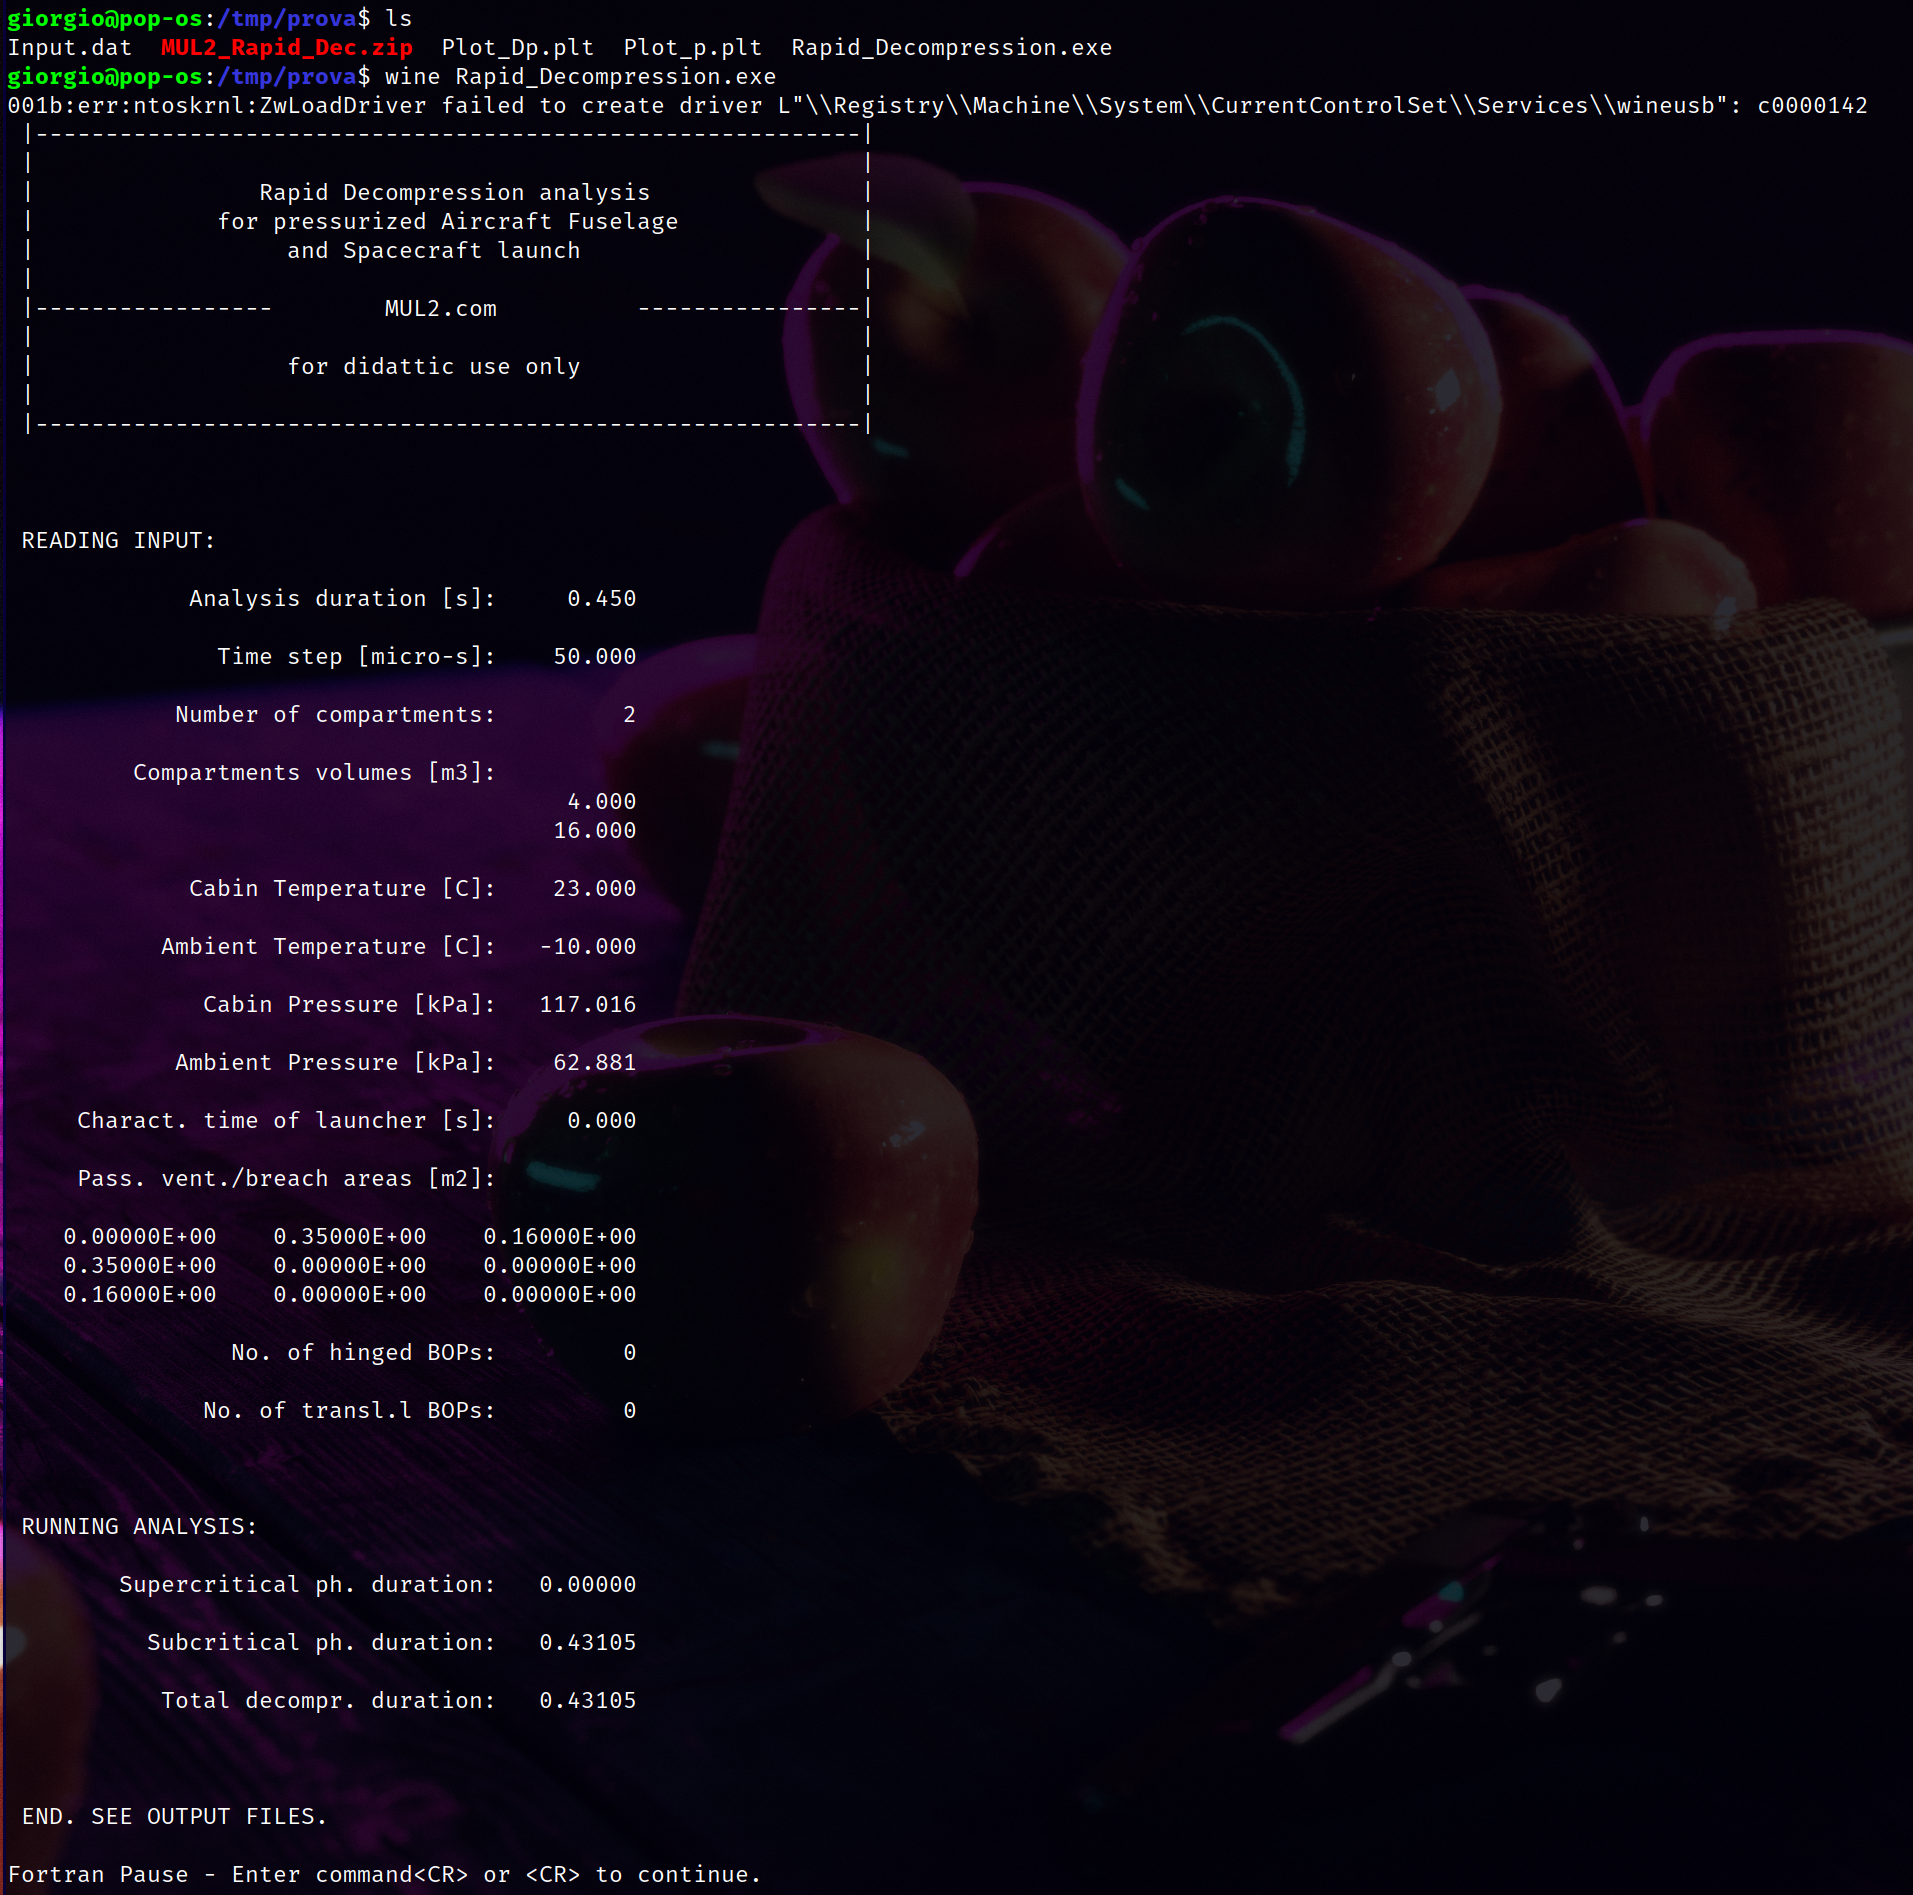
\includegraphics[width=\textwidth]{MUL2_feedback.png}\\
        \caption{stdout tipo}
    \end{figure}
    




        \clearpage
        \subsection{Esercizio 1\label{Es1}} 

        \begin{figure}[h!]
            \centering
            \phantomsection
            \label{fig:Esercizio_1}
            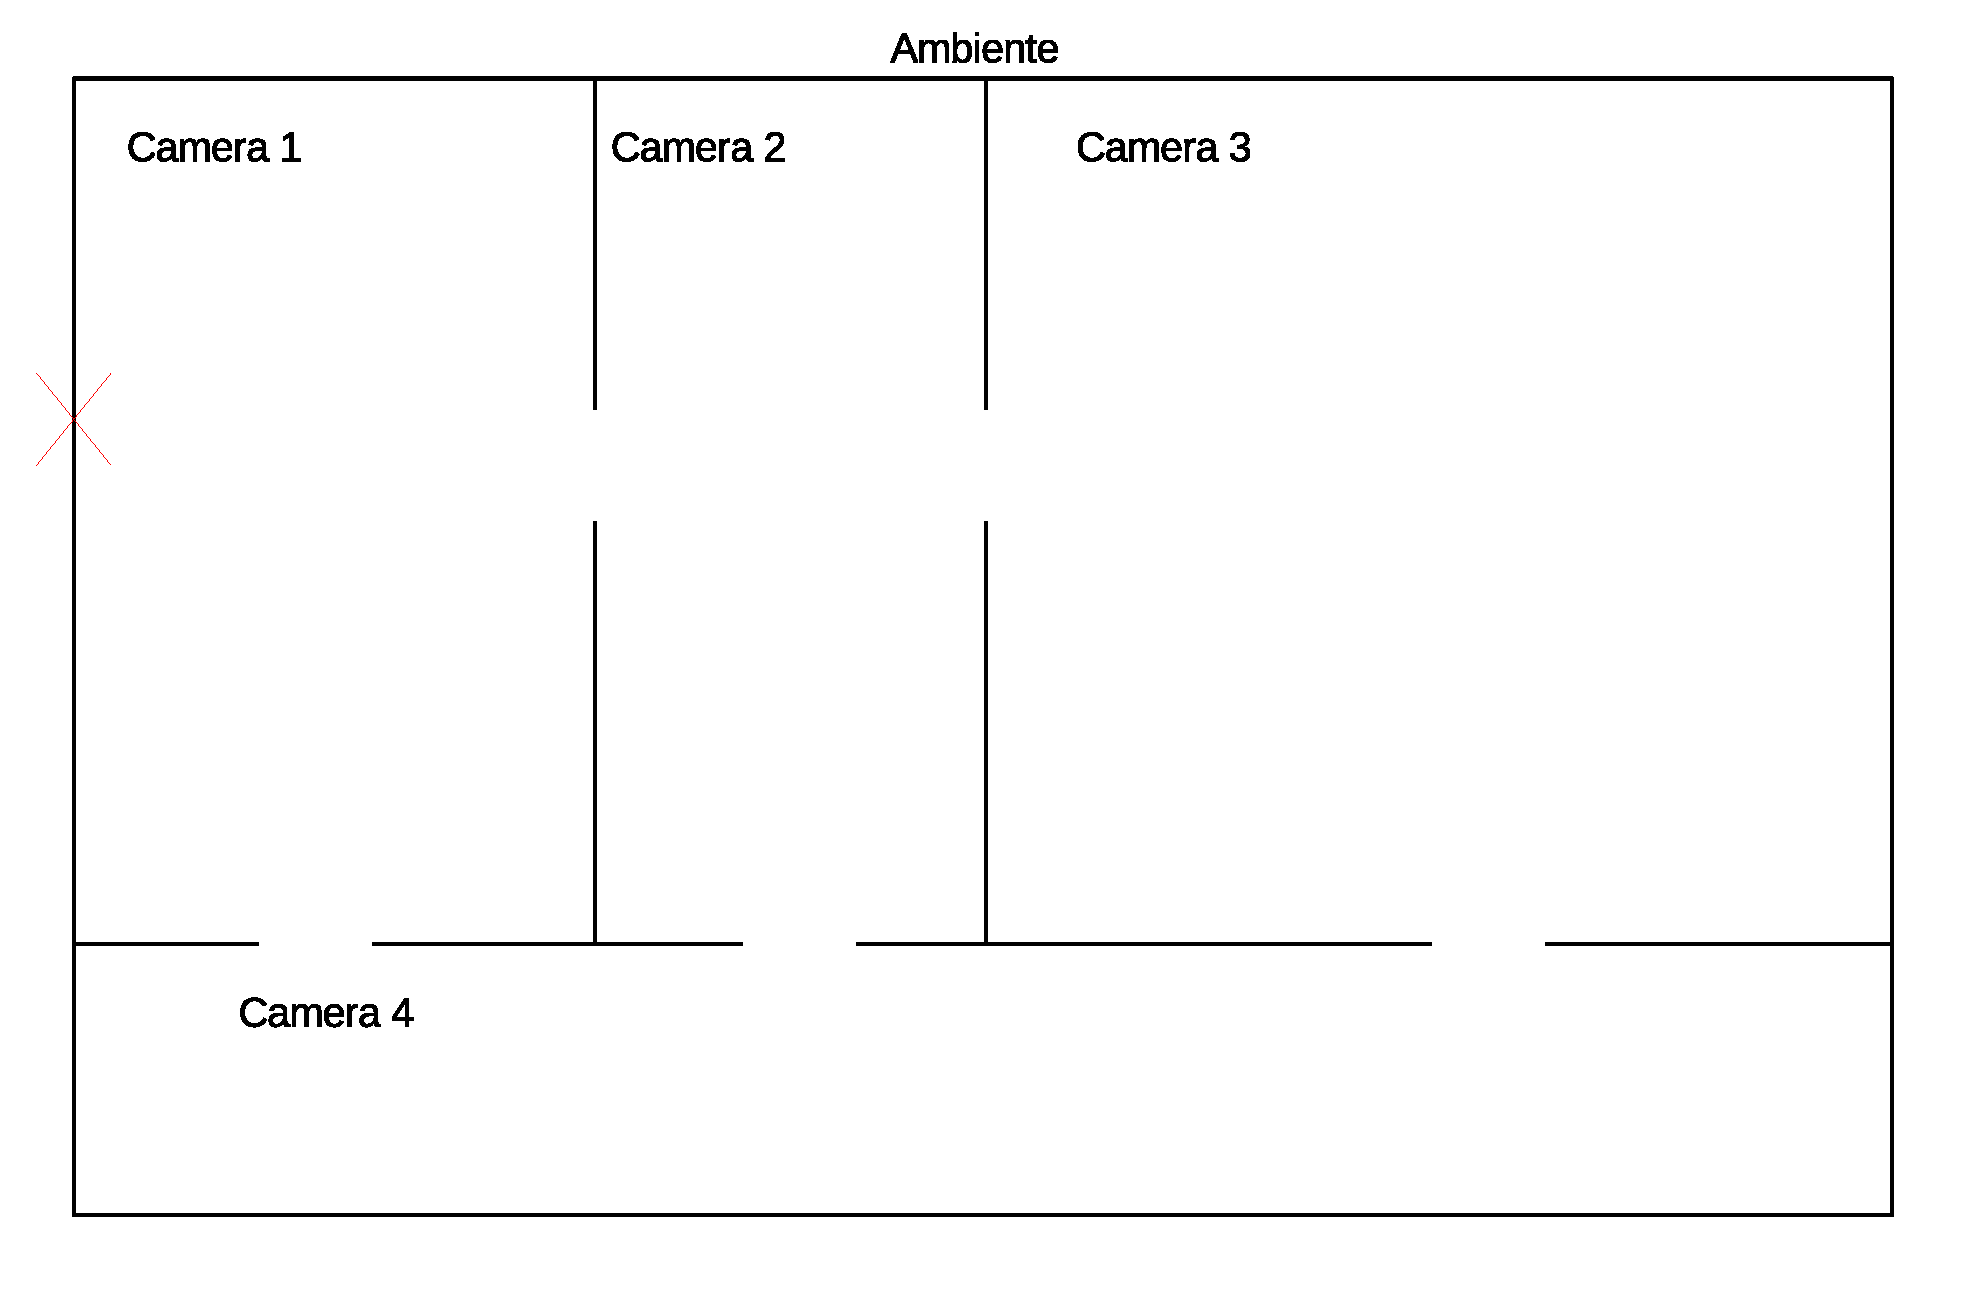
\includegraphics[width=0.5\textwidth]{ES1_Esercizio1.eps}
            \caption{Esercizio 1 (Disegnato con \textit{Inkscape} \autocite{Inkscape})}
        \end{figure}
        \subsubsection{DATI}
        \begin{itemize}
            \item $\displaystyle T_0 = -49.85\,°C;$ \
            \item $\displaystyle T_{c0} = 23\,°C;$ \
            \item $\displaystyle p_0 = 26.5\,kPa;$ \
            \item $\displaystyle p_{c0} = 89.876\,kPa;$ \
            \item $\displaystyle V_{C1} = 4\,m^3;$ \
            \item $\displaystyle V_{C2} = 3\,m^3;$ \
            \item $\displaystyle V_{C3} = 198\,m^3;$ \
            \item $\displaystyle V_{C4} = 67\,m^3;$ \
            \item $\displaystyle A_{1-0} = 1\,m^2;$ \
            \item $\displaystyle A_{1-2} = 0.6\,m^2;$ \
            \item $\displaystyle A_{2-3} = 0.6\,m^2;$ \
            \item $\displaystyle A_{1-4} = 0.8\,m^2;$ \
            \item $\displaystyle A_{3-4} = 0.8\,m^2;$ \
            \item $\displaystyle CD_{1-0} = 0.8;$ \
            \item $\displaystyle CD_{1-2} = [0, 0.5, 1];$ \
            \item $\displaystyle CD_{2-3} = 0.7;$ \
            \item $\displaystyle CD_{2-4} = 0.7;$ \
            \item $\displaystyle CD_{1-4} = 0.7;$ \
            \item $\displaystyle CD_{3-4} = 0.7;$ \
        \end{itemize}
        \clearpage
        \subsubsection{File di input}

        Il file di input viene modificato rispetto all'esempio, 
        inserendo ovviamente i dati forniti dal problema e rispettando la leggenda
        dello script.\\ 
        In particolare, la matrice delle aree effettive, ossia le singole aree fisiche che separano le camere, moltiplicate
        per i rispettivi coefficienti di efflusso, risulta: \\
        \begin{center}  
            \[
            \begin{pmatrix}
                0    & 0    & 0        & 0.56 & 0.8\\ 
                0    & 0    & 0.42     & 0.56 & 0\\ 
                0    & 0.42 & 0        & 0.56 & 0\\ 
                0.56 & 0.56 & 0.56     & 0    & 0\\
                0.8  & 0    & 0        & 0    & 0 
            \end{pmatrix}
            \]
            \\ 
            Per $\ CD_{1-2} = 0;$ \
            \\ 
            \[
            \begin{pmatrix}
                0    & 0.3  & 0        & 0.56 & 0.8\\ 
                0.3  & 0    & 0.42     & 0.56 & 0\\ 
                0    & 0.42 & 0        & 0.56 & 0\\ 
                0.56 & 0.56 & 0.56     & 0    & 0\\
                0.8  & 0    & 0        & 0    & 0 
            \end{pmatrix}
            \]
            \\ 
            Per $\ CD_{1-2} = 0.5;$ \
            \\ 
            \[
            \begin{pmatrix}
                0    & 0.6  & 0        & 0.56 & 0.8\\ 
                0.6  & 0    & 0.42     & 0.56 & 0\\ 
                0    & 0.42 & 0        & 0.56 & 0\\ 
                0.56 & 0.56 & 0.56     & 0    & 0\\
                0.8  & 0    & 0        & 0    & 0 
            \end{pmatrix}
            \]
            \\ 
            Per $\ CD_{1-2} = 1;$ \
        \end{center}    
        \clearpage

        \subsubsection{RISULTATI}
        Sono di seguito plottati gli andamenti delle pressioni e del 
        gradiente di pressione tra le camere 1 e 2, nel dominio del tempo. \\ 
        I plot sono ordinati a due a due per $\ CD_{1-2} = [0, 0.5, 1];$ \

        \begin{figure}[h!]
            \centering
            \phantomsection
            \label{fig:press_cam_0}
            \includegraphics[width=0.6\textwidth, angle=-90]{MUL2/Esercitazione1/1A/p.eps}
            \caption{Pressioni di entrambe le camere nel tempo, $t_{dec} = 3.28250 \ s$}
        \end{figure}

        \begin{figure}[h!]
            \centering
            \phantomsection
            \label{fig:grad_cam_0}
            \includegraphics[width=0.6\textwidth, angle=-90]{MUL2/Esercitazione1/1A/Dp.eps}
            \caption{Gradiente di pressione tra le due camere, $t_{dec} = 3.28250 \ s$}
        \end{figure}
        \clearpage
        
        \begin{figure}[h!]
            \centering
            \phantomsection
            \label{fig:press_cam_0.5}
            \includegraphics[width=0.6\textwidth, angle=-90]{MUL2/Esercitazione1/1B/p.eps}
            \caption{Pressioni di entrambe le camere nel tempo, $t_{dec} = 2.62989 \ s$}
        \end{figure}

        \begin{figure}[h!]
            \centering
            \phantomsection
            \label{fig:grad_cam_0.5}
            \includegraphics[width=0.6\textwidth, angle=-90]{MUL2/Esercitazione1/1B/Dp.eps}
            \caption{Gradiente di pressione tra le due camere, $t_{dec} = 2.62989 \ s$}
        \end{figure}
        \clearpage

        \begin{figure}[h!]
            \centering
            \phantomsection
            \label{fig:press_cam_1}
            \includegraphics[width=0.6\textwidth, angle=-90]{MUL2/Esercitazione1/1C/p.eps}
            \caption{Pressioni di entrambe le camere nel tempo, $t_{dec} = 2.42283 \ s$}
        \end{figure}

        \begin{figure}[h!]
            \centering
            \phantomsection
            \label{fig:grad_cam_1}
            \includegraphics[width=0.6\textwidth, angle=-90]{MUL2/Esercitazione1/1C/Dp.eps}
            \caption{Gradiente di pressione tra le due camere, $t_{dec} = 2.42283 \ s$}
        \end{figure}
        \clearpage

        \subsection{Esercizio 2\label{Es2}}

        Viene presa in analisi la depressurizzazione dell'\textit{UPM-Sat1} 
        \autocite{UPM_sat1}, in un tempo massimo di 225 s. \\ 

        \begin{figure}[h!]
            \centering
            \phantomsection
            \label{fig:MUL2_stdout}
            \includegraphics[width=0.5\textwidth]{MUL2/Esercitazione1/2A/Esercizio_2.eps}
            \caption{\textit{UPM-Sat1} (Disegnato con \textit{Inkscape} \autocite{Inkscape})}
        \end{figure}

        L'analisi é svolta assumendo un \textit{coefficiente di efflusso} unitario,
        rispettando inoltre il modello fornito di depressurizzazione della camera esterna: la pressione
        inizialmente ha un determinato valore, che non puó piú essere considerato costante come nei casi precedenti, ma avrá un andamento 
        esponenziale del tipo: \\
        \begin{equation}
            \phantomsection
            \label{equation_press_exp}
            \frac{p_e}{p_i} = e^{-\left ({\frac{t}{t_p}}  \right )^2}
        \end{equation}

        Dove $t_p$ é un tempo caratteristico, pari a 0.75 s in questo caso.
        \\ 
        \linebreak
        Infatti, mentre il volume esterno era assunto infinito per l'Esercizio 1 (\ref{Es1}), va chiaramente considerato
        finito in questo caso, con la conseguenza che la pressione diminuisce.
        \\ 
        \linebreak
        Il volume dell'unica camera considerata é pari a $0.13 \ m^3$, mentre 
        l'area che la separa dall'esterno é presa in tre valori test differenti, ossia:
        \[24 \cdot \begin{bmatrix}
            10^{-5}\ m^2\ & 10^{-6}\ m^2\ & 10^{-7} \ m^2\
            \end{bmatrix}\]
        \clearpage

        \subsection{RISULTATI\label{Esercizio2_risultati}}
        Anche in questo caso, sempre tramite lo script in Fortran fornito a lezione, 
        vengono calcolate le pressioni nel tempo e il gradiente di pressione $\Delta p$ agente sulle pareti
        del satellite, plottando poi il tutto con \textit{gnuplot}.\\ 
        I plot sono ordinati a due a due, per ogni area considerata.
        
        \begin{figure}[h!]
            \centering
            \includegraphics[width=0.5\textwidth, angle=-90]{MUL2/Esercitazione1/2A/p.eps}
            \phantomsection
            \label{fig:press_10_5}
            \caption{Andamento delle pressioni, $t_{subcritico} = 225.001  \ s$} 
        \end{figure}

        \begin{figure}[h!]
            \centering
            \includegraphics[width=0.5\textwidth, angle=-90]{MUL2/Esercitazione1/2A/Dp.eps}
            \phantomsection
            \label{fig:grad_press_10_5}
            \caption{Andamento del gradiente di pressione, $t_{subcritico} = 225.001  \ s$}
        \end{figure}


        \clearpage

        \begin{figure}[h!]
            \centering
            \includegraphics[width=0.6\textwidth, angle=-90]{MUL2/Esercitazione1/2B/p.eps}
            \phantomsection
            \label{fig:press_10_6}
            \caption{Andamento delle pressioni, $t_{subcritico} = 145.106  \ s$} 
        \end{figure}

        \begin{figure}[h!]
            \centering
            \includegraphics[width=0.6\textwidth, angle=-90]{MUL2/Esercitazione1/2B/Dp.eps}
            \phantomsection
            \label{fig:grad_press_10_6}
            \caption{Andamento del gradiente di pressione, $t_{subcritico} = 145.106  \ s$}
        \end{figure}
        \clearpage

        \begin{figure}[h!]
            \centering
            \includegraphics[width=0.6\textwidth, angle=-90]{MUL2/Esercitazione1/2C/p.eps}
            \phantomsection
            \label{fig:press_10_7} 
            \caption{Andamento delle pressioni, $t_{subcritico} = 69.735  \ s$}
        \end{figure}
        
        \begin{figure}[h!] 
            \centering
            \includegraphics[width=0.6\textwidth, angle=-90]{MUL2/Esercitazione1/2C/Dp.eps}
            \phantomsection
            \label{fig:grad_press_10_7}
            \caption{Andamento del gradiente di pressione, $t_{subcritico} = 69.735  \ s$}
        \end{figure}

        \clearpage

        \subsection{Riflessioni}
        Dal primo Esercizio (\ref{Es1}), prendendo in analisi le prime due camere, si puó immediatamente notare come,
        a paritá di condizioni e di area comunicante tra i due volumi,
        il coefficiente di efflusso giochi un ruolo importante nel determinare l'andamento
        delle pressioni nelle due camere e, di conseguenza, il gradiente di pressione tra le due,
        a sua volta origine di carichi agenti sulla parete.\\ 
        Sono stati considerati tre casi, ossia il caso limite di efflusso nullo, quello di efflusso totale
        ed un caso intermedio.\\ 
        Nel caso di efflusso nullo (\ref{fig:press_cam_0}), la pressione decresce
        vertiginosamente entro pochi istanti nella prima stanza, con un picco piú elevato 
        rispetto agli altri casi, dopodiché resta costante, mentre nella seconda camera
        si ha una decrescita lineare piú lenta fino ad un picco piú basso che negli altri casi.\\ 
        Considerando un efflusso intermedio (\ref{fig:press_cam_0.5}), si puó giá 
        notare come la pressione nella prima camera decresca sí rapidamente, ma 
        fino ad un valore di picco meno elevato, per poi stabilizzarsi brevemente e riprendere con una decrescita molto lenta, 
        mentre nella seconda camera si ha una decrescita piú rapida del caso precedente e fino ad un valore di picco piú alto.
        \\ 
        Il trend é ancora piú evidente se si prende in considerazione un efflusso 
        totale (\ref{fig:press_cam_1}): la pressione della prima camera
        raggiunge un picco ancora piú basso e tende a decrescere un po' piú rapidamente
        dopo una breve stabilizzazione, ma comunque entro valori piú bassi dei casi precedenti, mentre 
        la seconda camera vede una decrescita di pressione ancora piú rapida
        e fino ad un picco piú alto.\linebreak
        \linebreak
        Quindi, dato che il gradiente é semplicemente calcolato come il valore assoluto
        della differenza tra i due profili di pressione, si nota immediatamente che, 
        all'aumentare del coefficiente di efflusso da 0 a 1, il suo valore
        massimo si minimizza e si ottiene anche una decrescita piú rapida.\\ 
        Da ció si deduce che, avere un efflusso troppo basso (o, peggio ancora, nullo)
        tra cabina e altri compartimenti in presenza di una breccia verso l'ambiente esterno, genera dei carichi di sollecitazione
        piú elevati, con possibili danni strutturali catastrofici.

        \clearpage

        
        Nel secondo Esercizio (\ref{Es2}), il coefficiente di efflusso viene assunto unitario
        ed il focus é sull'area che separa i due ambienti studiati.\\ 
        Nello specifico, vengono ancora una volta analizzate le pressioni tra le camere, 
        al fine di studiarne l'andamento del gradiente di pressione, 
        mettendo in risalto l'influenza che l'area di comunicazione puó avere.\\ 
        Il valore é ridotto, progressivamente nei tre casi,
        di un ordine di grandezza.\\ \linebreak
        Nel primo caso in questione, i due profili di pressione sono pressappoco identici (si ricorda che il modello utilizzato 
        é esponenziale (\ref{equation_press_exp})), per cui il gradiente ha un valore di picco molto basso (\ref{fig:grad_press_10_5}).\\ 
        Nel secondo caso l'area si riduce di un ordine di grandezza: i due profili
        di pressione cominciano a differenziarsi in maniera piú evidente per la scala studiata,
        ed il gradiente assume, come logico aspettarsi, un andamento analogo al precedente ma con un massimo significativamente
        piú elevato, di ben due ordini di grandezza per la precisione (\ref{fig:grad_press_10_6}).\\ 
        Nell'ultimo caso, l'area viene ulteriormente ridotta di un altro ordine di grandezza:
        stavolta gli andamenti delle pressioni si discostano sostanzialmente, con un decadimento
        molto piú rapido per la seconda camera.\\ 
        Di conseguenza, il gradiente risultante, pur mantenendo lo stesso tipo di 
        andamento, é cresciuto ulteriormente di un ordine di grandezza (\ref{fig:grad_press_10_7}).\\ 
        
    

        Si puó quindi intuire che, in una situazione di depressurizzazione, il ruolo dell'area di efflusso sia fondamentale
        nel tenere sotto controllo i carichi dovuti al gradiente di pressione: un'area troppo piccola
        potrebbe creare un gradiente eccessivamente alto e potenzialmente pericoloso per le
        strutture coinvolte.
        \clearpage
        \section{Esercitazione 2\label{Esercitazione_2}}

        Lo scopo di questa esercitazione é l'analisi modale di un sistema a quattro gradi di libertá,
        composto da quattro masse discretizzate, rappresentanti i due stage, il faring ed il payload 
        di un lanciatore che ricalca il \textit{Falcon 9}. Le varie masse sono connesse da molle e smorzatori viscosi, questi
        ultimi trascurati per semplificare il modello matematico.

        Inoltre, la spinta nei primi 160 secondi é ipotizzata costante, utilizzando
        un modello con carico a gradino.

        \begin{figure}[h!]
            \centering
            \phantomsection
            \label{fig:esercitazione2_drawing}
            
\includegraphics[width=0.8\textwidth]{MUL2/Esercitazione2/Esercitazione2.eps}
            \caption{Lanciatore (Disegnato con \textit{Inkscape} \autocite{Inkscape})}
        \end{figure}

        \subsection{Dati\label{Esercitazione_2_dati}}

        \begin{itemize}
            \item $m_{1\rightarrow 4} = \left\{445, \ 116, \ 2, \ 15\right\} \cdot 10^3 \ kg  $
            \item $k_{1\rightarrow 3} = \left\{5, \ 5, \ 1 \right\} \cdot 10^8 \frac{N}{m} $
            \item $c_{1\rightarrow 3} \approx \left\{0, \ 0, \ 0 \right\}$
            \item $F_0 = 775 \cdot 10^3 \ kg_f$
            \item $t_{launch} = 160 \ s$
        \end{itemize}
        \clearpage

        \subsection{Frequenze naturali e modi propri di vibrare\label{Esercitazione_2_modi}}

        Si considera inizialmente un sistema con equazioni di equilibrio accoppiate, in forma omogenea, ossia con vettore
        delle forze applicate nullo. In notazione matriciale: 

            \begin{equation}
                \phantomsection \label{equation:sist_omogeneo}
                M\ddot{x} + Kx(t) = 0
            \end{equation}
        dove M e K sono rispettivamente le matrici delle masse concentrate e di rigidezza, cosí definite:
        \begin{center}  
            \[
            \begin{pmatrix}
                m_1    & 0    & 0     & 0 \\ 
                0      & m_2  & 0     & 0 \\
                0      & 0    & m_3   & 0 \\
                0      & 0    & 0     & m_4 
                
            \end{pmatrix}
            \]
            \\ 
            \[
            \begin{pmatrix}
                k_1    & -k_1       & 0                     & 0 \\ 
                -k_1   & k_1 + k_2  & -k_2                  & 0 \\
                0      & -k_2       & k_2 + k_3             & -k_3 \\
                0      & 0          & -k_3                  & k_3 
                
            \end{pmatrix}
            \]
            
        \end{center}    
    
        La soluzione omogenea é chiaramente un \textit{moto armonico}, non smorzato e privo di forzante.
        Rappresenta un classico problema agli autovalori, risolto in uno script su \textit{Octave} \autocite{Octave}, disponibile 
        nel repository di questo report \autocite{Esercitazioni_strutture}, col nome di \textit{Esercitazione2.m} e comprendente
        la risoluzione del resto di questa esercitazione.

        Oltre alla soluzione banale, si ottiene il vettore degli autovalori, da cui sono ricavate le pulsazioni e
        le frequenze naturali del sistema, oltre alla matrice contenente tutti e quattro i vettori modali in colonna.

        \begin{equation}
            \phantomsection \label{equation:puls_nat}
            \vec{\omega}_n  = \left[0.0000, \ 63.2520, \ 87.4808, \ 552.0482 \right] \ rad \cdot s^{-1} 
        \end{equation}

        \begin{equation}
            \phantomsection \label{equation:freq_nat}
            \vec{f}_n  = \left[0.0000, \ 10.0669, \ 13.9230, \ 87.8612 \right] \ Hz 
        \end{equation}

        \begin{equation}
            \phantomsection \label{equation:matrice_modale}
         \Phi = \begin{pmatrix}
                   0.0013   & -0.0006       & -0.0004             &  0.0000     \\ 
                   0.0013   & 0.0016        &  0.0021             &  0.0003     \\
                   0.0013   & 0.0023        &  0.0008             & -0.0222    \\
                   0.0013   & 0.0059        & -0.0055             &  0.0005
                \end{pmatrix} 
        \end{equation}

        \clearpage

        \subsection{Grandezze generalizzate\label{Esercitazione_2_grandezze_generalizzate}}

        Si passa quindi alla risoluzione del sistema completo, utilizzando questa volta 
        le incognite modali, che permettono di riscrivere il sistema con delle grandezze generalizzate.
        
        Vale la relazione $x(t) = \phi q(t)$, per cui il sistema risulta:

        \begin{equation}
            \phantomsection \label{equation:sistema_generalizzato}
            M_g \ddot{q}(t) + K_g q(t) = F_g
        \end{equation}

        in cui $M_g \ , \ K_g \ e \ F_g$ sono rispettivamente la matrice delle masse, la matrice delle rigidezze
        ed il vettore delle forze applicate in forma generalizzata. \\ 

        Tali grandezze sono quindi calcolate dallo script \autocite{Esercitazioni_strutture} e sono pari a:

            \begin{equation}
                \phantomsection \label{equation:masse_generalizzate}
                M_g = 
                \begin{pmatrix}
                   1        & 0             &  0             &  0     \\ 
                   0        & 1             &  0             &  0     \\
                   0        & 0             &  1             &  0    \\
                   0        & 0             &  0             &  1
                \end{pmatrix} kg
            \end{equation} \\ 


            \begin{equation}
                \phantomsection \label{equation:rigidezze_generalizzate}
                K_g = 
                \begin{pmatrix}
                   0        & 0             &  0             &  0     \\ 
                   0        & 0.0400        &  0             &  0     \\
                   0        & 0             &  0.0765        &  0     \\
                   0        & 0             &  0             &  3.0476
                \end{pmatrix} \cdot 10^5 \ \frac{N}{m}
            \end{equation} \\ 


            \begin{equation}
                \phantomsection \label{equation:forze_generalizzate}
                F_g = 
                \begin{pmatrix}
                   1             \\ 
                  -0.4762        \\
                  -0.2686        \\
                  -0.009        
                \end{pmatrix} \cdot 10^4 \ N
            \end{equation}

        La matrice delle masse generalizzate coincide con la matrice identitá, per cui l'algoritmo
        utilizzato dalla funzione \textit{eig(K, M)} garantisce degli autovettori M-normalizzati.

        A questo punto, il sistema di equazioni accoppiate a quattro gradi di libertá é scorporato in quattro equazioni armoniche
        indipendenti ad un grado di libertá, grazie al principio di sovrapposizione. 
        
        In questo modo, 
        la risoluzione viene notevolmente semplificata, pur utilizzando un sistema del tutto equivalente
        a quello di partenza. 

        \clearpage

        \subsection{Calcolo dei displacement verticali delle quattro masse\label{Esercitazione_2_displacement}}

        Sempre attraverso lo stesso script \autocite{Esercitazioni_strutture}, vengono calcolate le quattro componenti
        del vettore displacement $\vec{x}(t)$, a partire dal vettore modale $\vec{q}(t)$.

        Data la natura semplificata del problema, si ricavano facilmente due soluzioni analitiche per la prima e per le restanti componenti:

            \begin{equation}
                \phantomsection \label{equation:q1}
                q_1 = \frac{F_{g1}}{2M_{g1}} \ t^2
            \end{equation}

            \begin{equation}
                \phantomsection \label{equation:q1}
                q_i = \frac{F_{g_i}}{K_{g_i}} \ \left[1 - cos\left(\omega_{n_i} t\right) \right] 
            \end{equation}

        Viene quindi plottato l'andamento del vettore nel tempo:

            \begin{figure}[h!]
                \phantomsection \label{fig:displacement_x}
                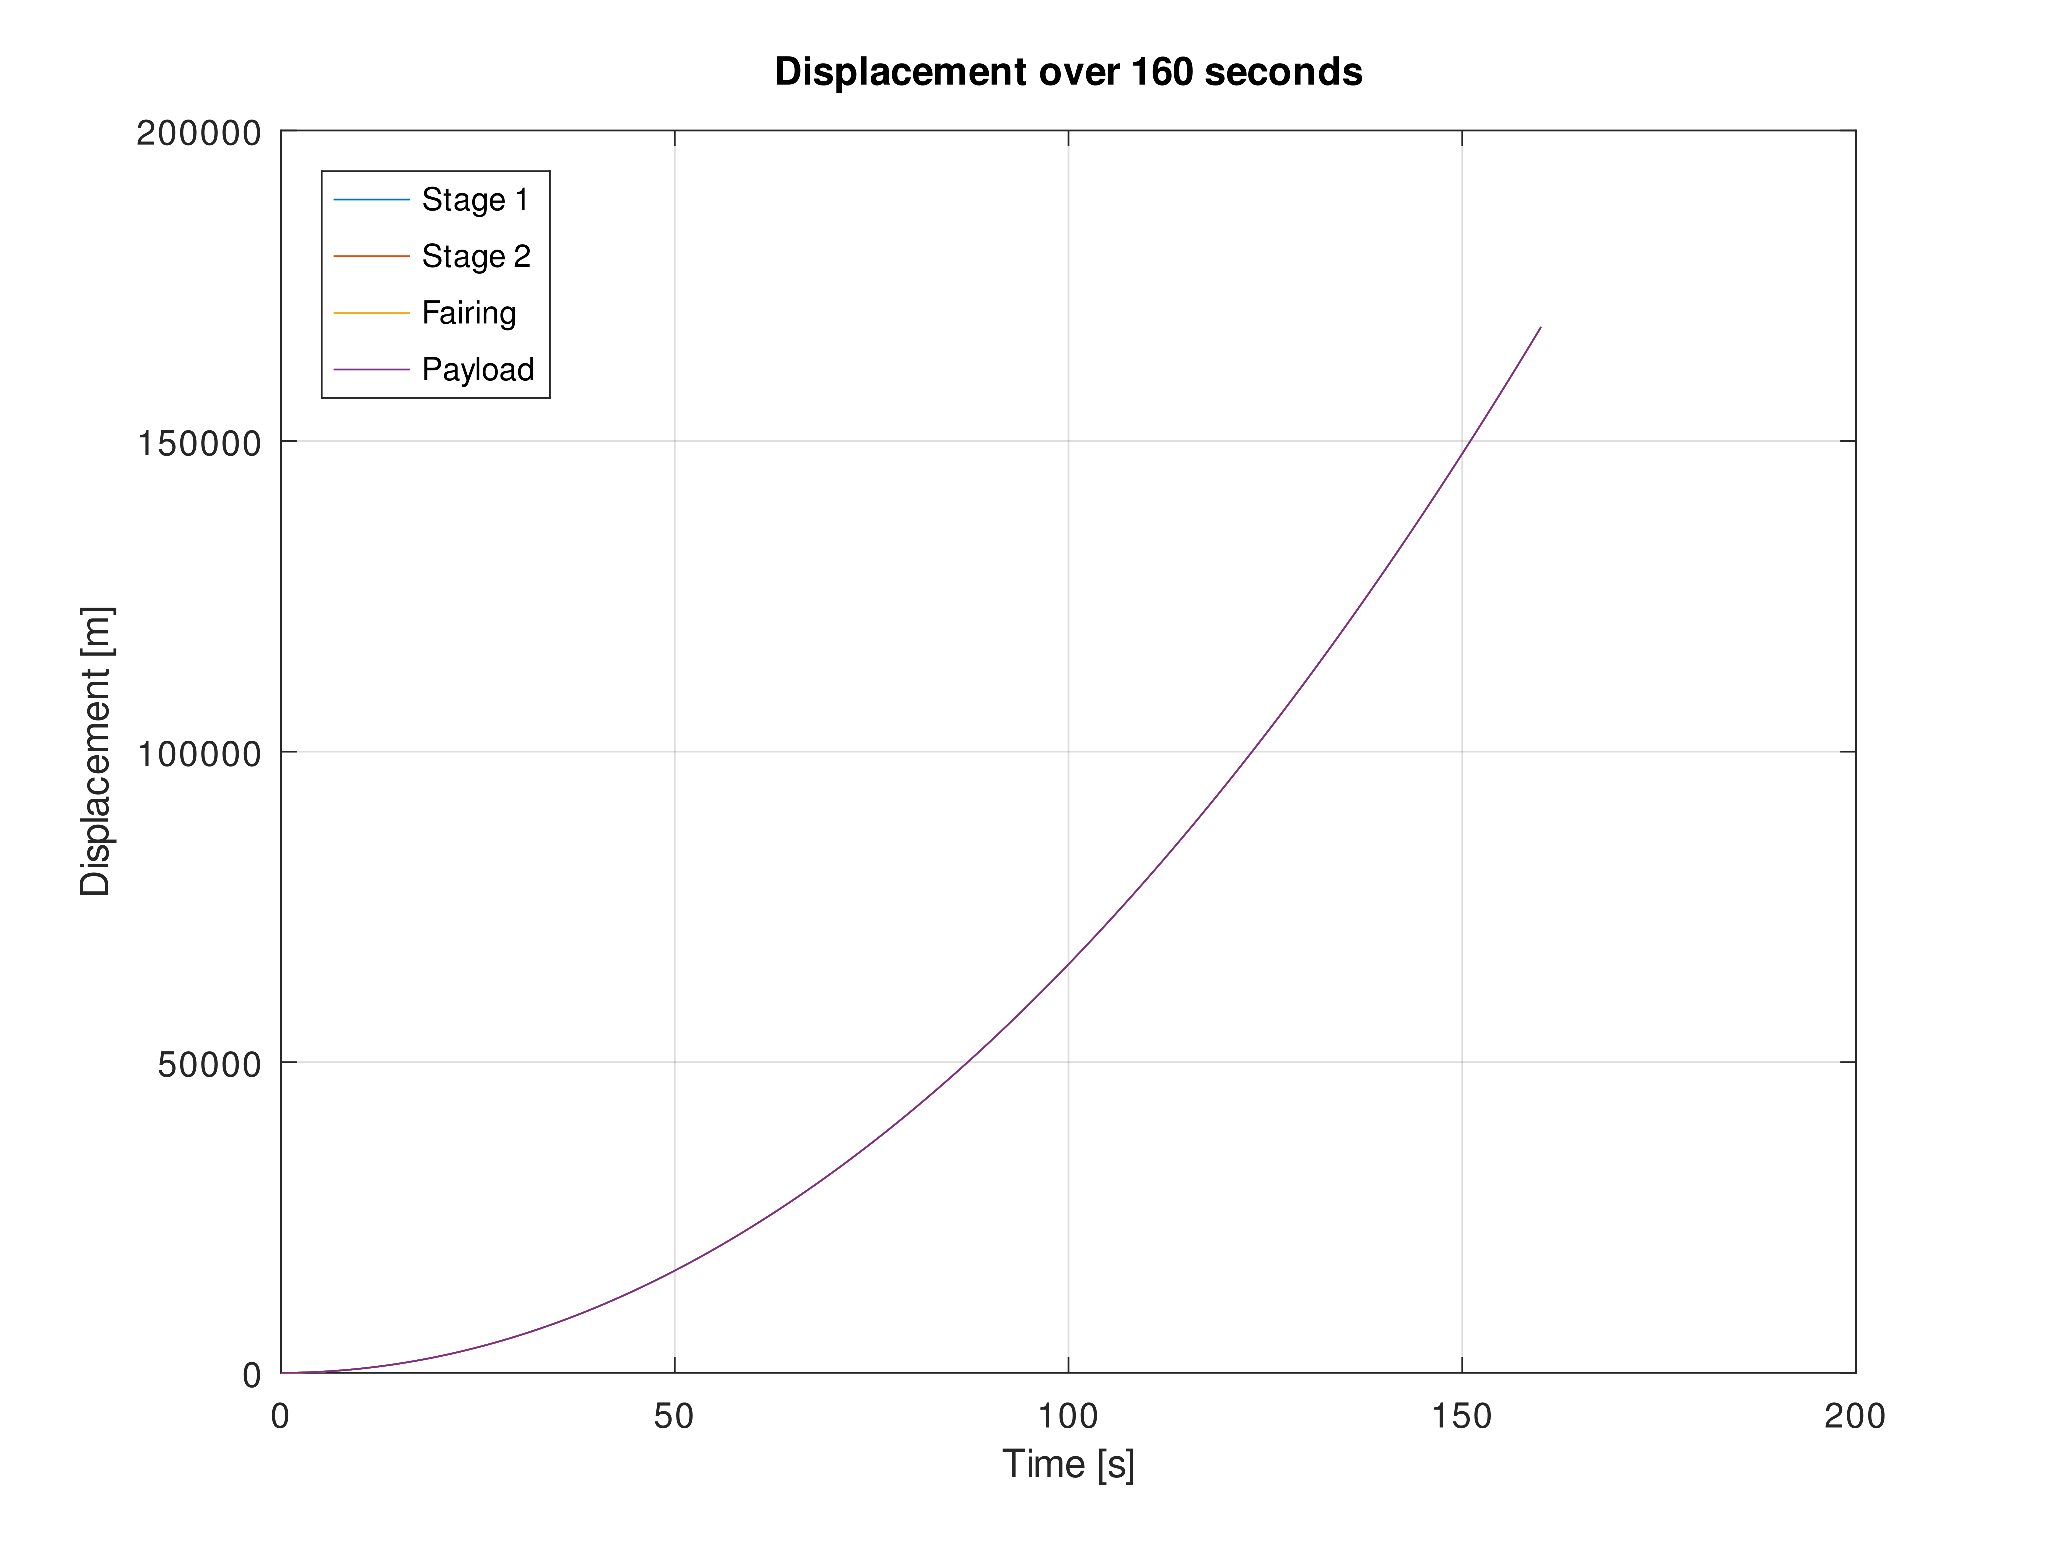
\includegraphics[width=0.5\textwidth]{MUL2/Esercitazione2/Matlab/disp_160.eps}
                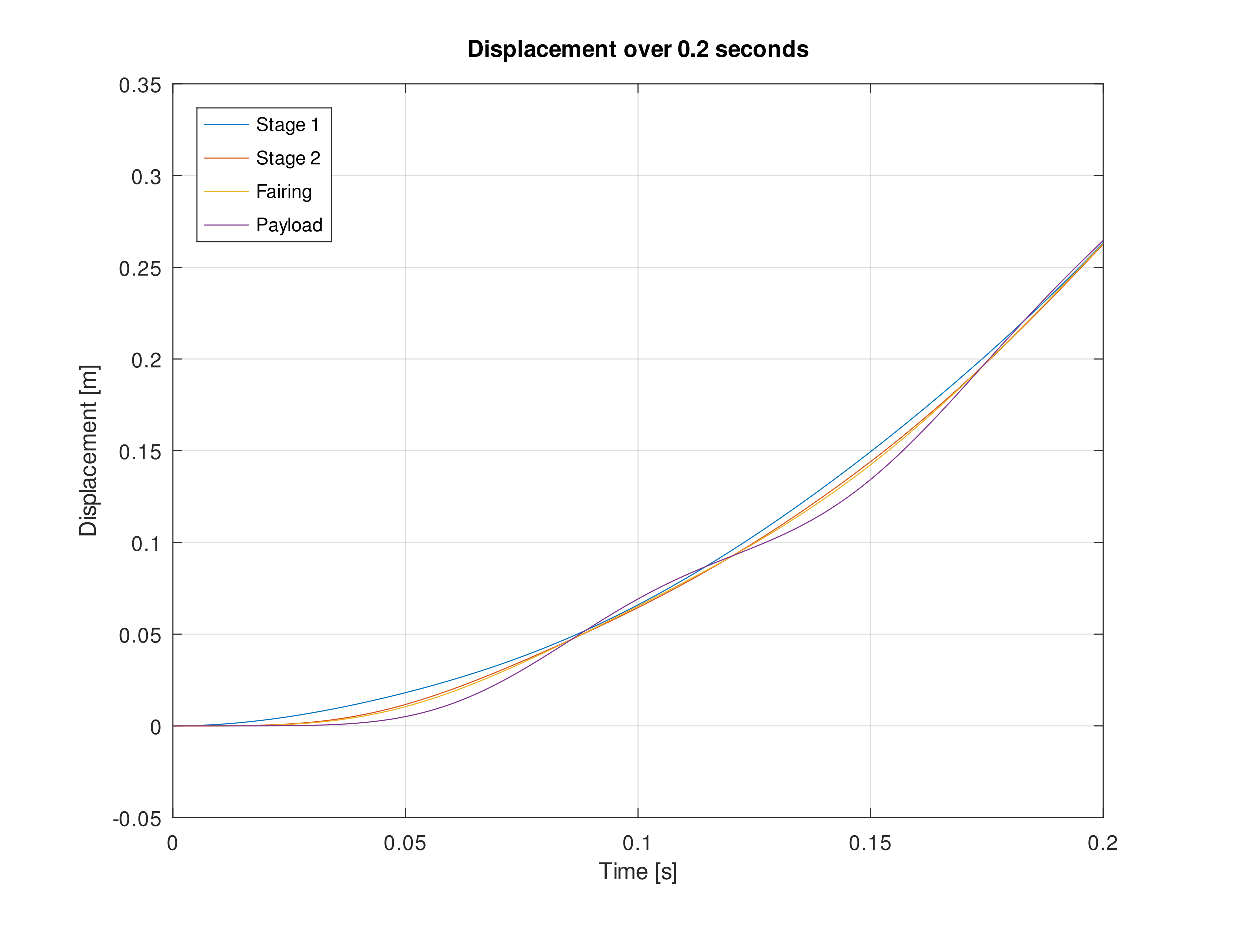
\includegraphics[width=0.5\textwidth]{MUL2/Esercitazione2/Matlab/disp_0.2.eps}
                \caption{Displacement per 160 s e per 0.2 s}
            \end{figure}
        
        Si puó notare come, su un tempo sufficientemente lungo, l'andamento delle quattro masse sia praticamente coincidente.
        Per la durata molto breve del lift-off, invece, si nota che l'andamento delle varie parti 
        si discosta leggermente, con particolare enfasi per il payload, che subisce delle oscillazioni particolarmente
        evidenti, motivo per cui é necessario studiare accuratamente in fase progettuale questo transitorio, 
        onde evitare potenziali danni ad attrezzature estremamente costose e spesso molto soggette a starature, se sottoposte a variazioni
        repentine di questo tipo.

        \clearpage

        \subsection{Accelerazione e carico trasmessi al payload\label{Esercitazione_2_acc_load}}

        In virtú di quanto detto in sezione \ref{Esercitazione_2_displacement}, si calcolano anche i 
        vettori accelerazione e carico tra 0 e 2 secondi, con particolare attenzione all'andamento del payload.

        \begin{figure}[h!]
            \phantomsection \label{fig:acc_load}
            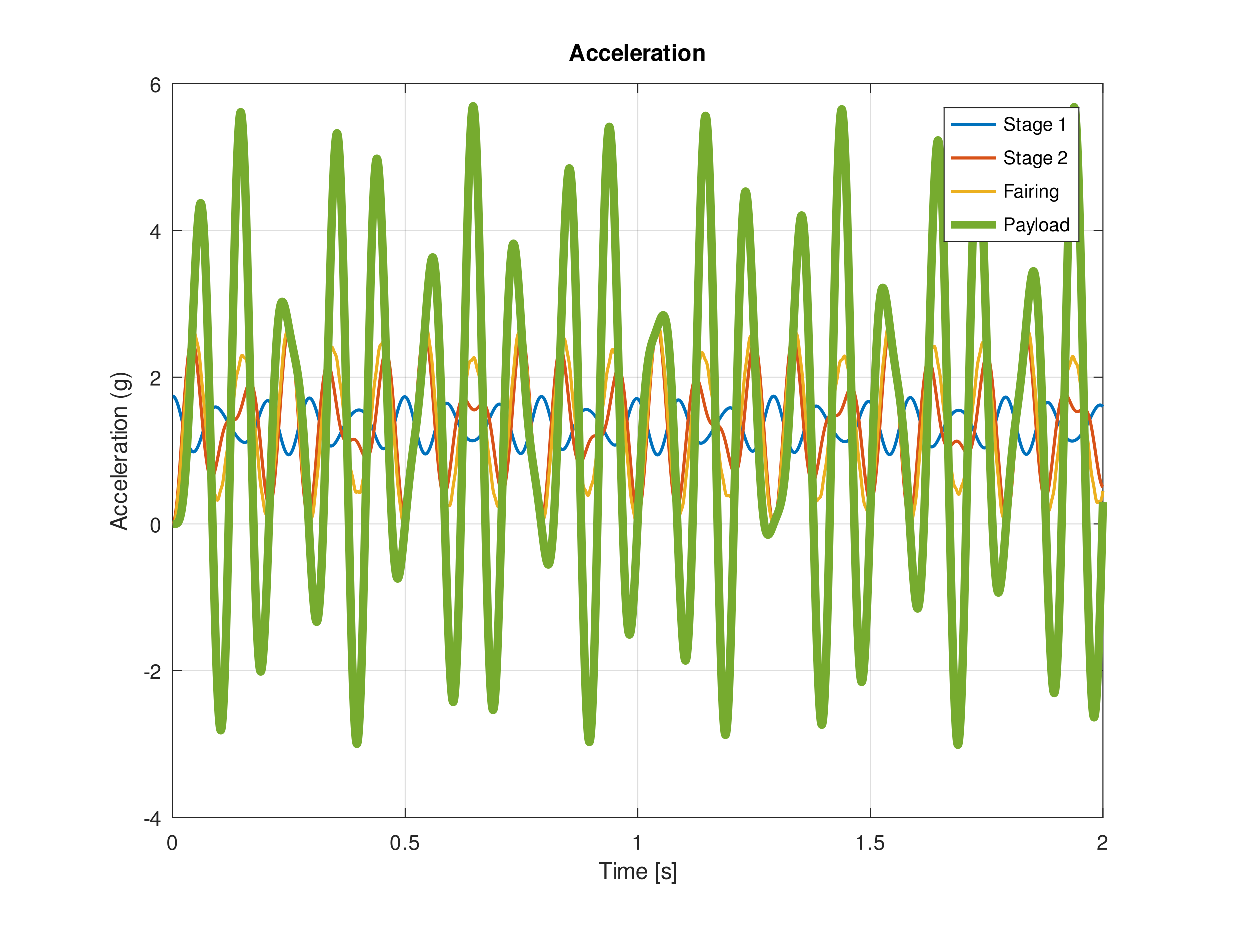
\includegraphics[width=0.5\textwidth]{MUL2/Esercitazione2/Matlab/acceleration.eps}
            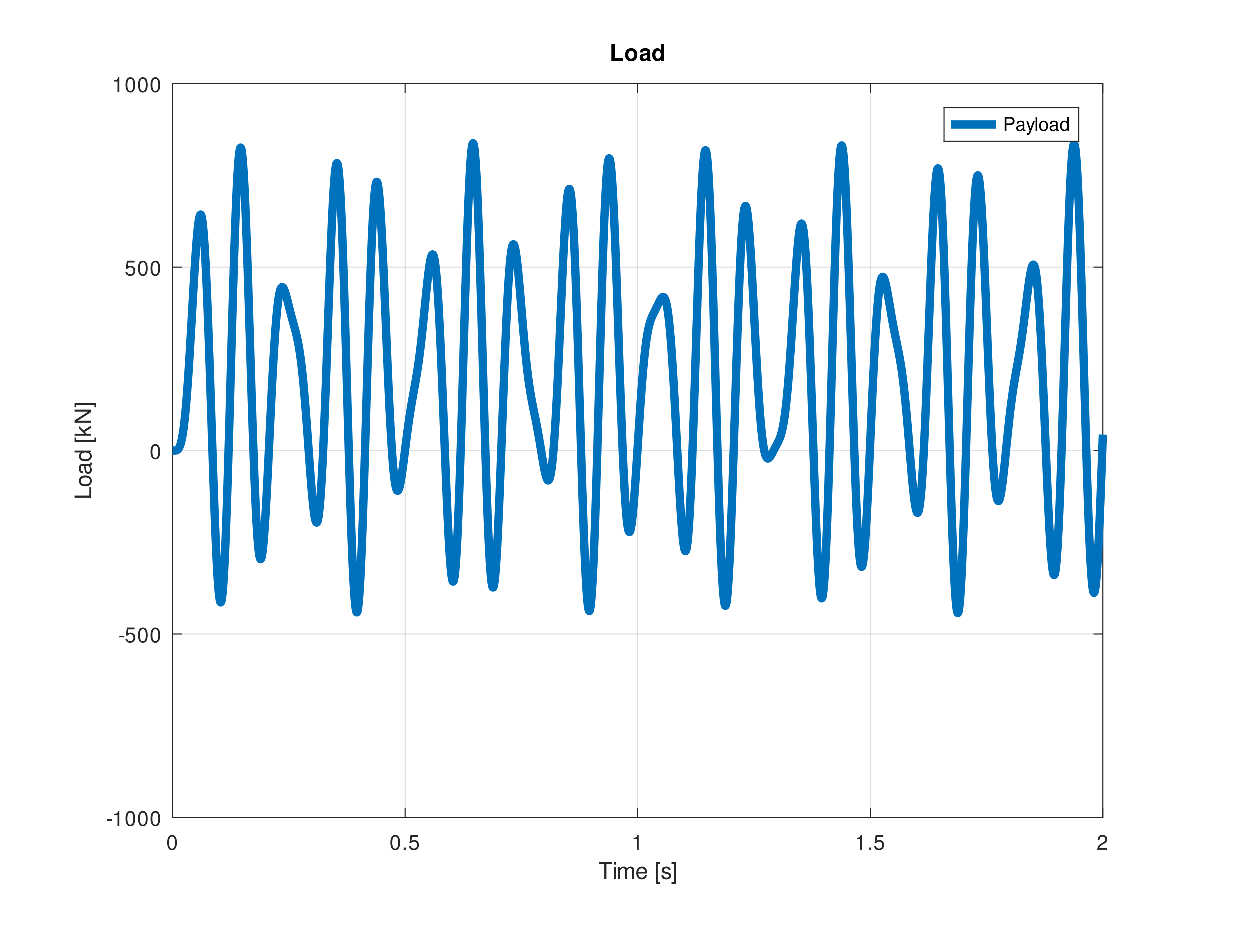
\includegraphics[width=0.5\textwidth]{MUL2/Esercitazione2/Matlab/load.eps}
            \caption{Accelerazioni e carico sul payload, tra 0 e 2 s}
        \end{figure}

        Come detto in precedenza, il payload é spesso molto sensibile a oscillazioni cosí notevoli di 
        accelerazioni (e dei carichi che ne derivano, ottenuti riscalando le accelerazioni per un fattore pari alla massa), 
        specie nel caso di payload ottici. 

        Si possono osservare picchi estremamente alti, fino a 6g, che dovrebbero essere assolutamente ridotti
        in fase di progettazione, tenendo anche in considerazione che é necessario ideare un sistema
        posizionamento ed ancoraggio del payload ottimale. \\ 

        Va peró tenuto a mente che il problema é stato notevolmente semplificato, proprio a partire da un'assunzione
        estremamente forte, ossia la rimozione dei coefficienti di smorzamento viscoso.

        Naturalmente, in una situazione piú realistica, la presenza di meccanismi assimilabili a smorzatori 
        é assolutamente d'obbligo, per cui le forti oscillazioni osservate finora sono senz'altro una grossa
        sovrastima, dato che verrebbero smorzate in maniera efficiente, in un progetto reale.

        \clearpage
        
        \subsection{Power Spectral Density dell'accelerazione\label{Esercitazione_2_PSD}}

        A questo punto si calcola la \textit{Power Spectral Density} dell'accelerazione $\ddot{x}_4 (t)$, che rappresenta la potenza 
        distribuita su un dominio scomposto di frequenze. \\ 

        Nello script si utilizza la funzione \textit{periodogram} per valutare la PSD, di seguito plottata.

            \begin{figure}[h!]
                \phantomsection \label{fig:PSD}
                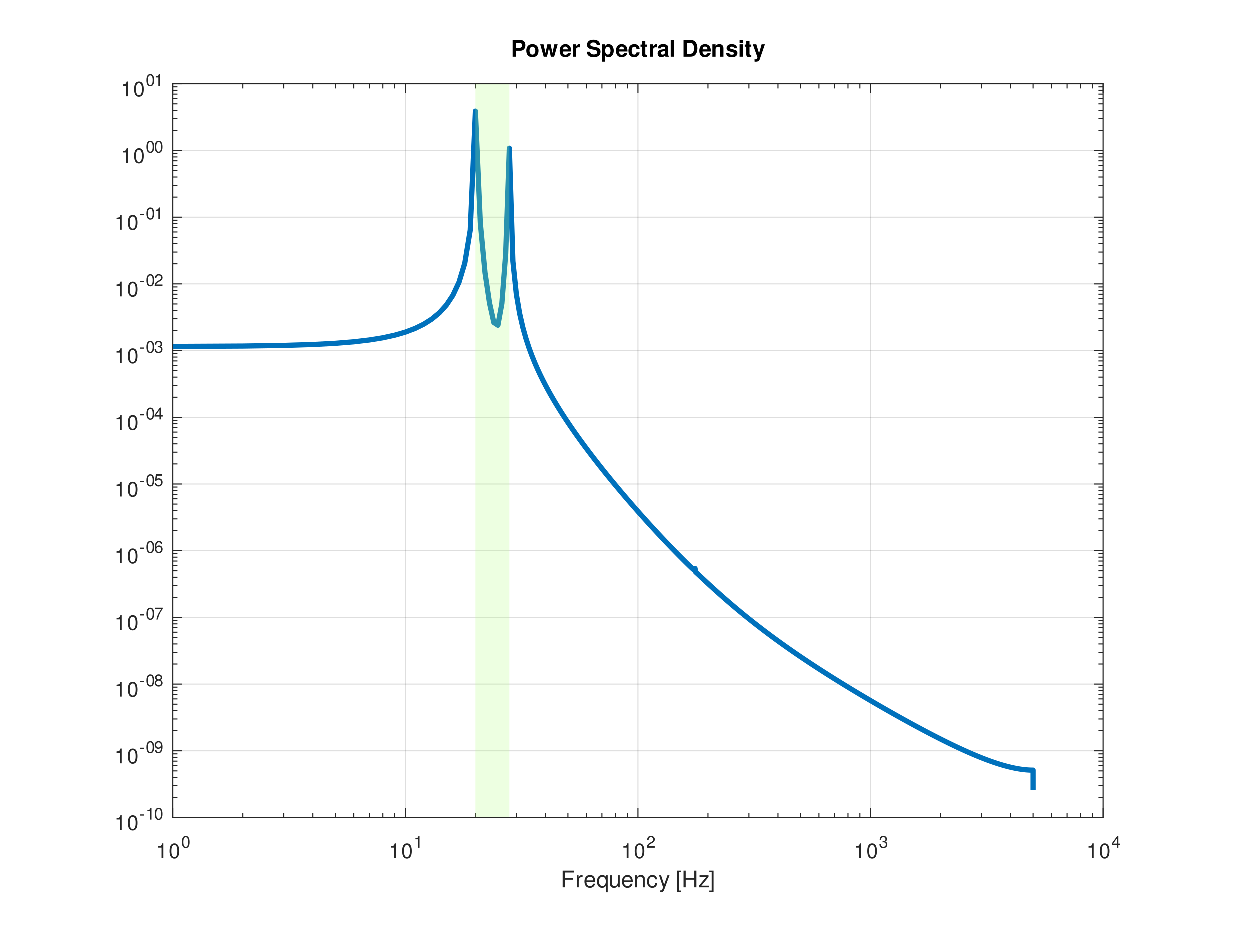
\includegraphics[width=\textwidth]{MUL2/Esercitazione2/Matlab/PSD.eps}
                \caption{Power Spectral Density dell'accelerazione del payload}
            \end{figure}

        Si possono osservare due picchi compresi tra i 20 Hz e i 30 Hz, per i quali si hanno i maggiori valori di potenza. \\ 

        Si é quindi calcolato un valore quadratico medio pari a $\ddot{x}_{4,rms} = 24.3278 \ g$.

        \clearpage

        \section{Esercitazione 3 \label{Esercitazione_3}}

            \begin{figure}[h!]
                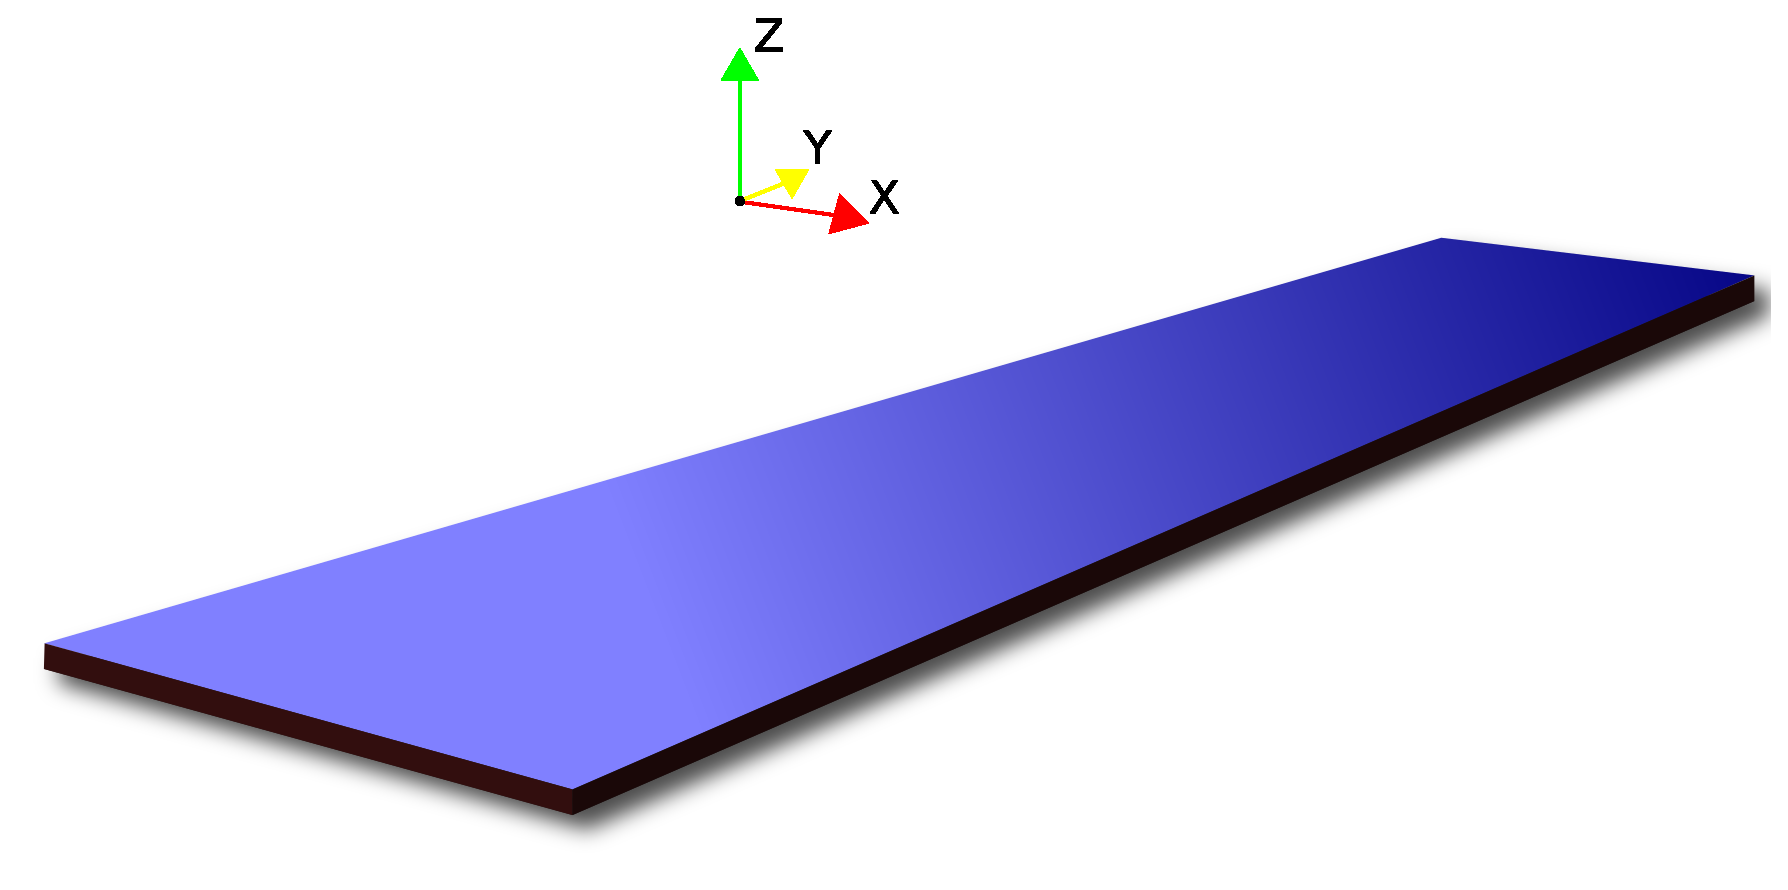
\includegraphics[width=\textwidth]{MUL2/Esercitazione3/plank.eps}
                \caption{Piastra incastrata ad una delle estremitá}
            \end{figure}

        Lo scopo di questa esercitazione é lo svolgimento di un'analisi FEM di una piastra incastrata su uno 
        dei lati corti, di cui si valuteranno i risultati ottenuti.

            \subsection{Dati\label{Esercitazione3_dati}}

            \begin{itemize}
                \item $Dim = \left\{1, \ 0.2, \ 0.006 \right\} \ m $
                \item $\alpha_{layers} = \left\{0, \ 90, \ 0 \right\} \ \deg \  \wedge \  \left\{0, \ 45, \ 0 \right\} \ \deg$
                \item $t_{single \ layer} = 0.002 \ m$
                \item $\vec{E}_{1\rightarrow 3} = \left\{138, \ 9.5, \ 9.5\right\} \ GPa $
                \item $\vec{G} = \left\{G_{12}, \ G_{13}, \ G_{23}\right\} = \left\{5.2, \ 5.2, \ 1.45\right\} \ GPa$
                \item $\vec{\nu } = \left\{\nu_{12}, \ \nu_{13}, \ \nu_{23}\right\} = \left\{0.28, \ 0.28, \ 0.4\right\}$
                \item $\rho = 1570 \frac{kg}{m^3}$ (Materiale omogeneo e ad alto grado di ortotropia)
            \end{itemize}

            \clearpage

            \subsection{Frequenze naturali e modi propri di vibrare \label{Esercitazione3_freq_nat}}

            Tramite uno script in Fortran fornito a lezione \autocite{MUL2}, che utilizza vari file di input testuale, \
            si calcolano le prime dieci frequenze naturali della struttura. \\ 

            L'algoritmo in questo caso utilizzato implementa una discretizzazione in 31 nodi indipendenti (10 elementi con 4 nodi longitudinali, 9 nodi trasversali per layer, 
            6 nodi condivisi tra strati adiacenti), sfruttando un'analisi \textit{layer wise} con modello LE (lagrangiano).

            \subsubsection{Laminazione a 90 gradi \label{Esercitazione3_freq_nat_90}}

                \begin{table}[h!]
                    \centering
                    \begin{tabular}{@{}ll@{}}
                    \toprule
                    $f_1$    & 0.894014303E+01  \ Hz \ (flex) \\
                    $f_2$    & 0.323353291E+02  \ Hz \ (torque) \\
                    $f_3$    & 0.558631886E+02  \ Hz \ (flex) \\
                    $f_4$    & 0.108330254E+03  \ Hz \ (torque) \\
                    $f_5$    & 0.155727004E+03  \ Hz \ (flex) \\
                    $f_6$    & 0.215825295E+03  \ Hz \ (torque) \\
                    $f_7$    & 0.220986476E+03  \ Hz \ (flex) \\
                    $f_8$    & 0.303227073E+03  \ Hz \ (flex) \\
                    $f_9$    & 0.365244247E+03  \ Hz \ (flex) \\
                    $f_{10}$ & 0.497030995E+03  \ Hz \ (torque) \\ \bottomrule
                \end{tabular}
                \caption{Frequenze naturali}
                \label{tab:freq_nat}
                \end{table}
            
            In seguito, con il software open-source \textit{Paraview} \autocite{Paraview}, estremamente versatile nel postprocessing dei dati, 
            sono state visualizzate le deformazioni dovute ai dieci modi propri di vibrare, di seguito riportati 
            (in ordine, prima tutti i gradi flessionali e poi quelli torsionali). 

            \clearpage

            \begin{figure}[h!]
                \phantomsection \label{fig:freq_nat_flex_90}
                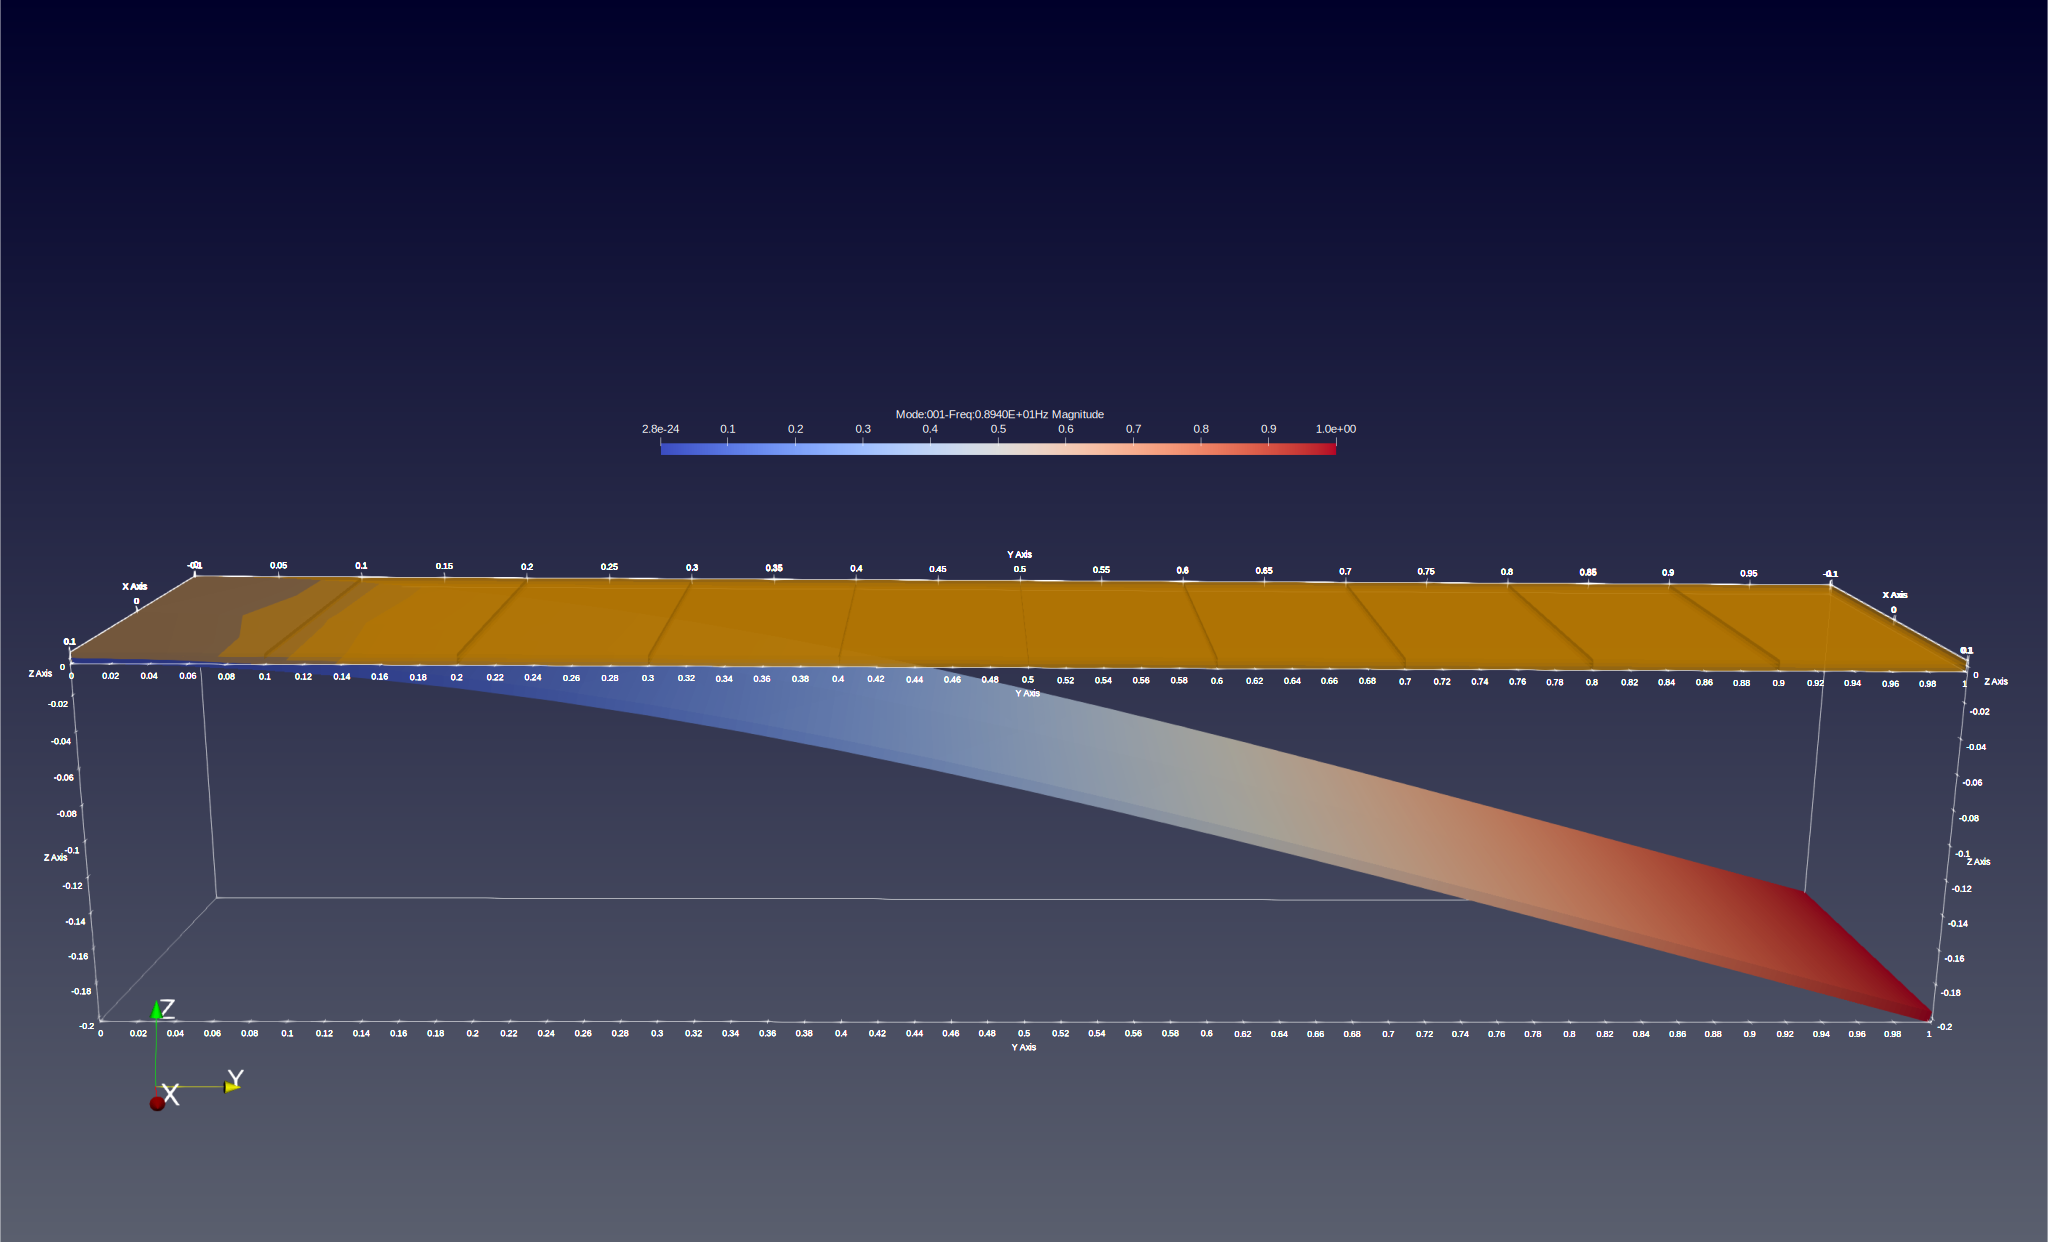
\includegraphics[width=0.5\textwidth]{MUL2/Esercitazione3/MUL2_FEM/OUTPUT/dynamic/90deg/Flex/flex1.eps}
                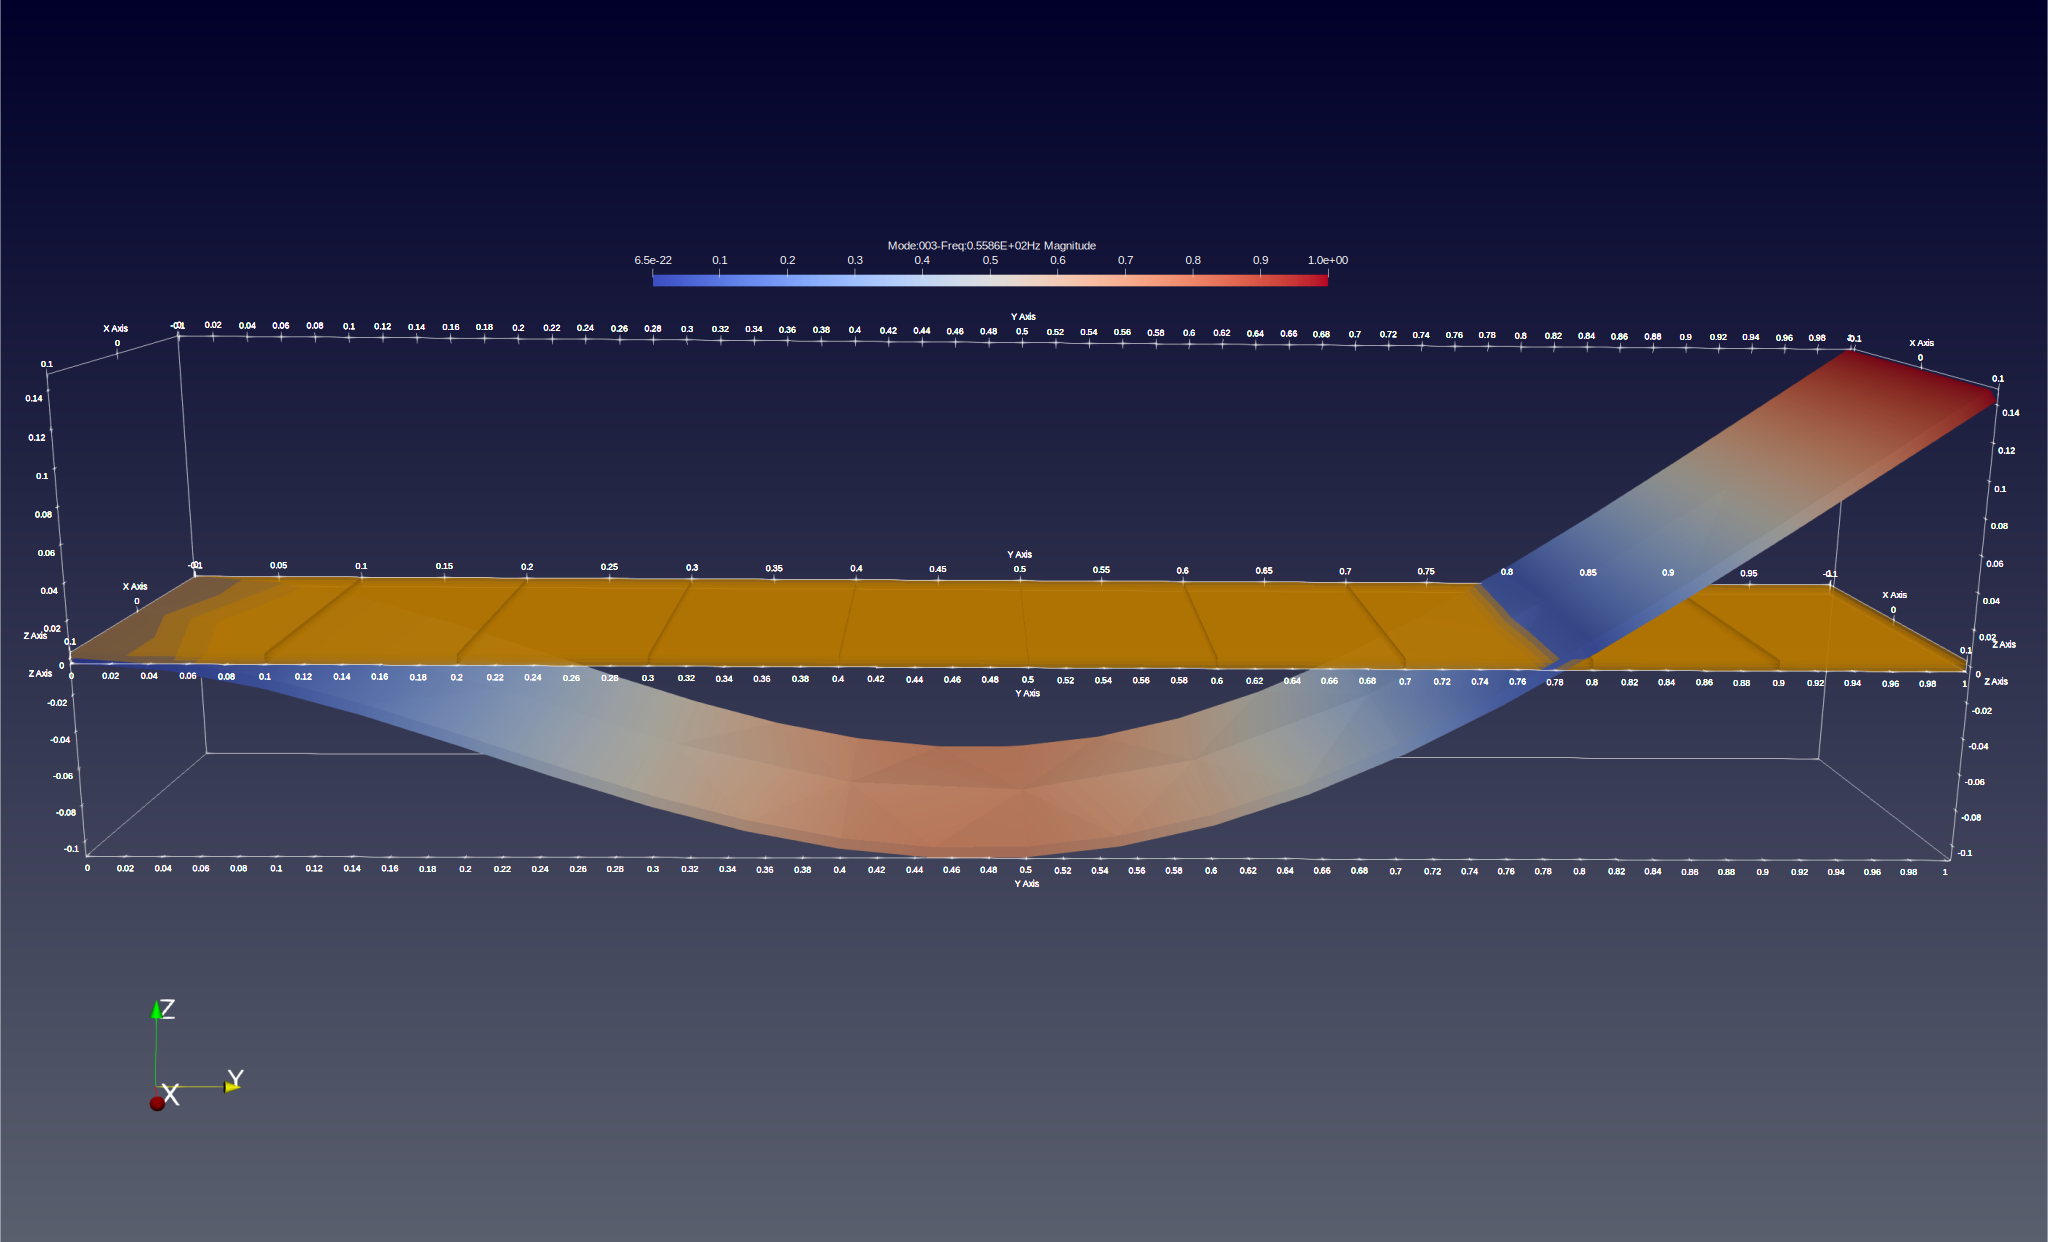
\includegraphics[width=0.5\textwidth]{MUL2/Esercitazione3/MUL2_FEM/OUTPUT/dynamic/90deg/Flex/flex2.eps}
                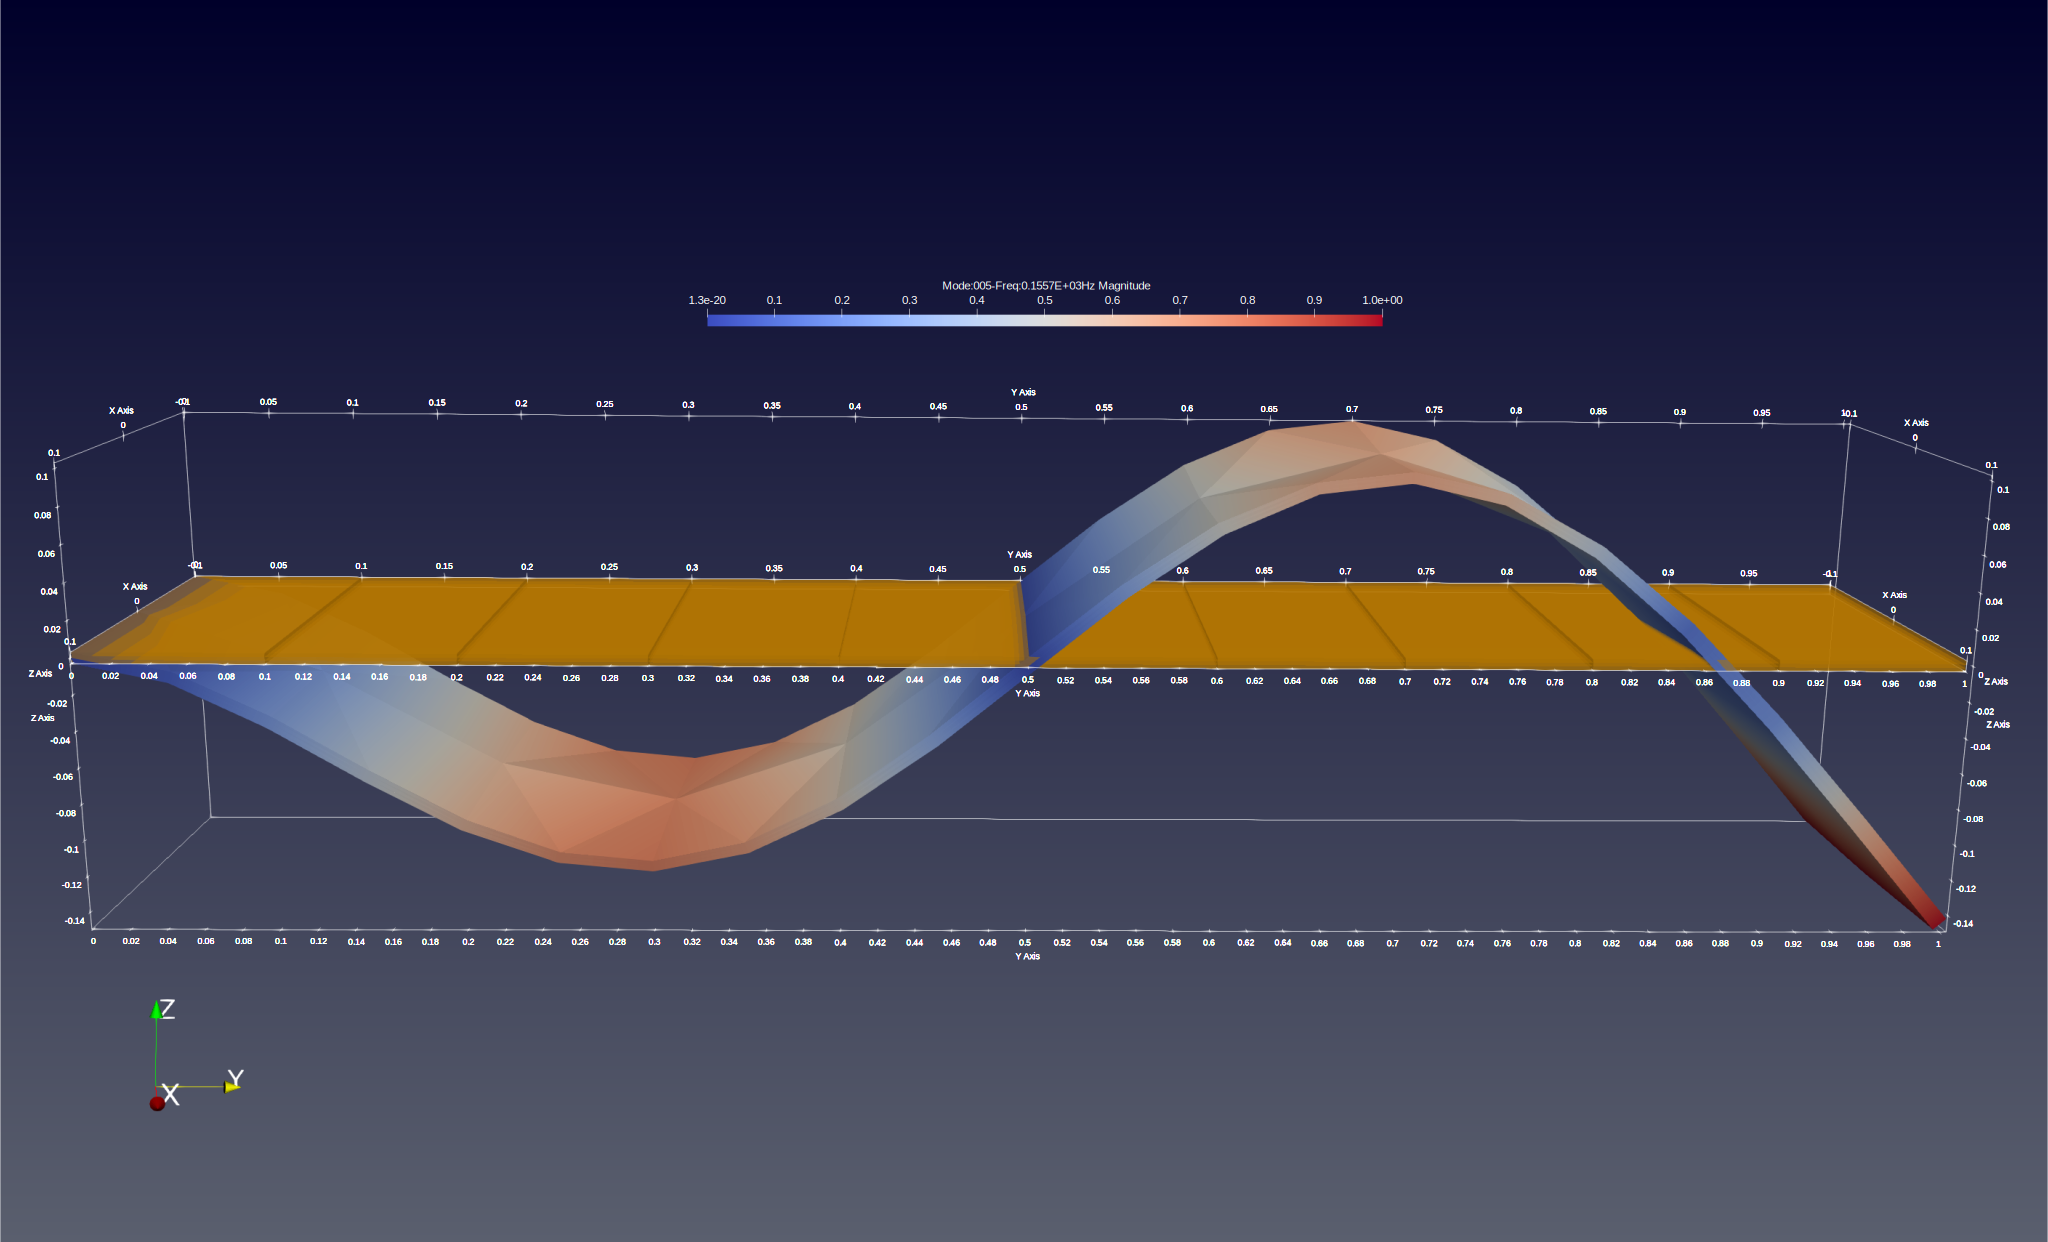
\includegraphics[width=0.5\textwidth]{MUL2/Esercitazione3/MUL2_FEM/OUTPUT/dynamic/90deg/Flex/flex3.eps}
                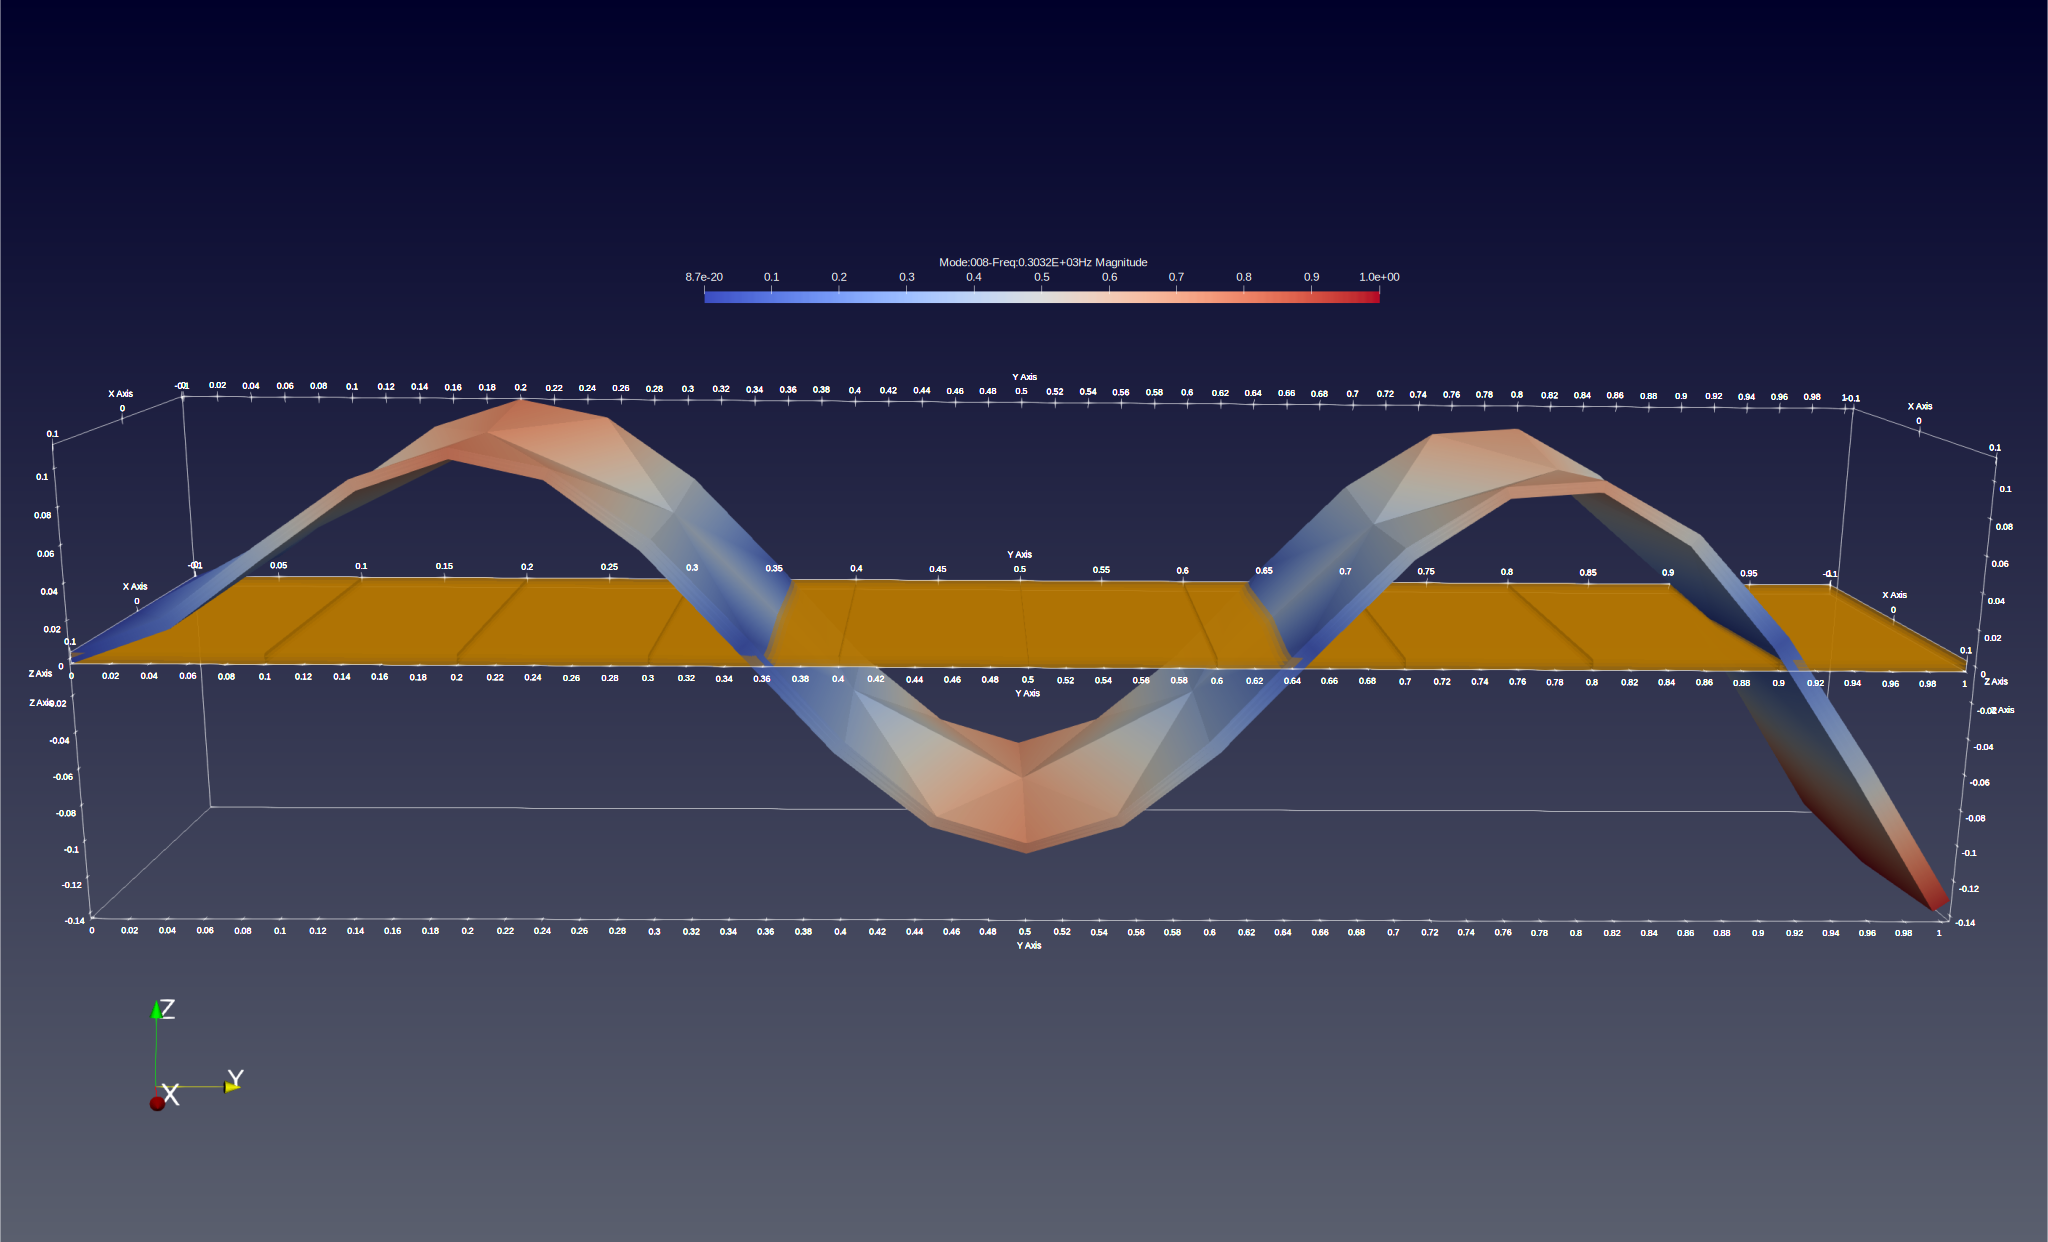
\includegraphics[width=0.5\textwidth]{MUL2/Esercitazione3/MUL2_FEM/OUTPUT/dynamic/90deg/Flex/flex4.eps}
                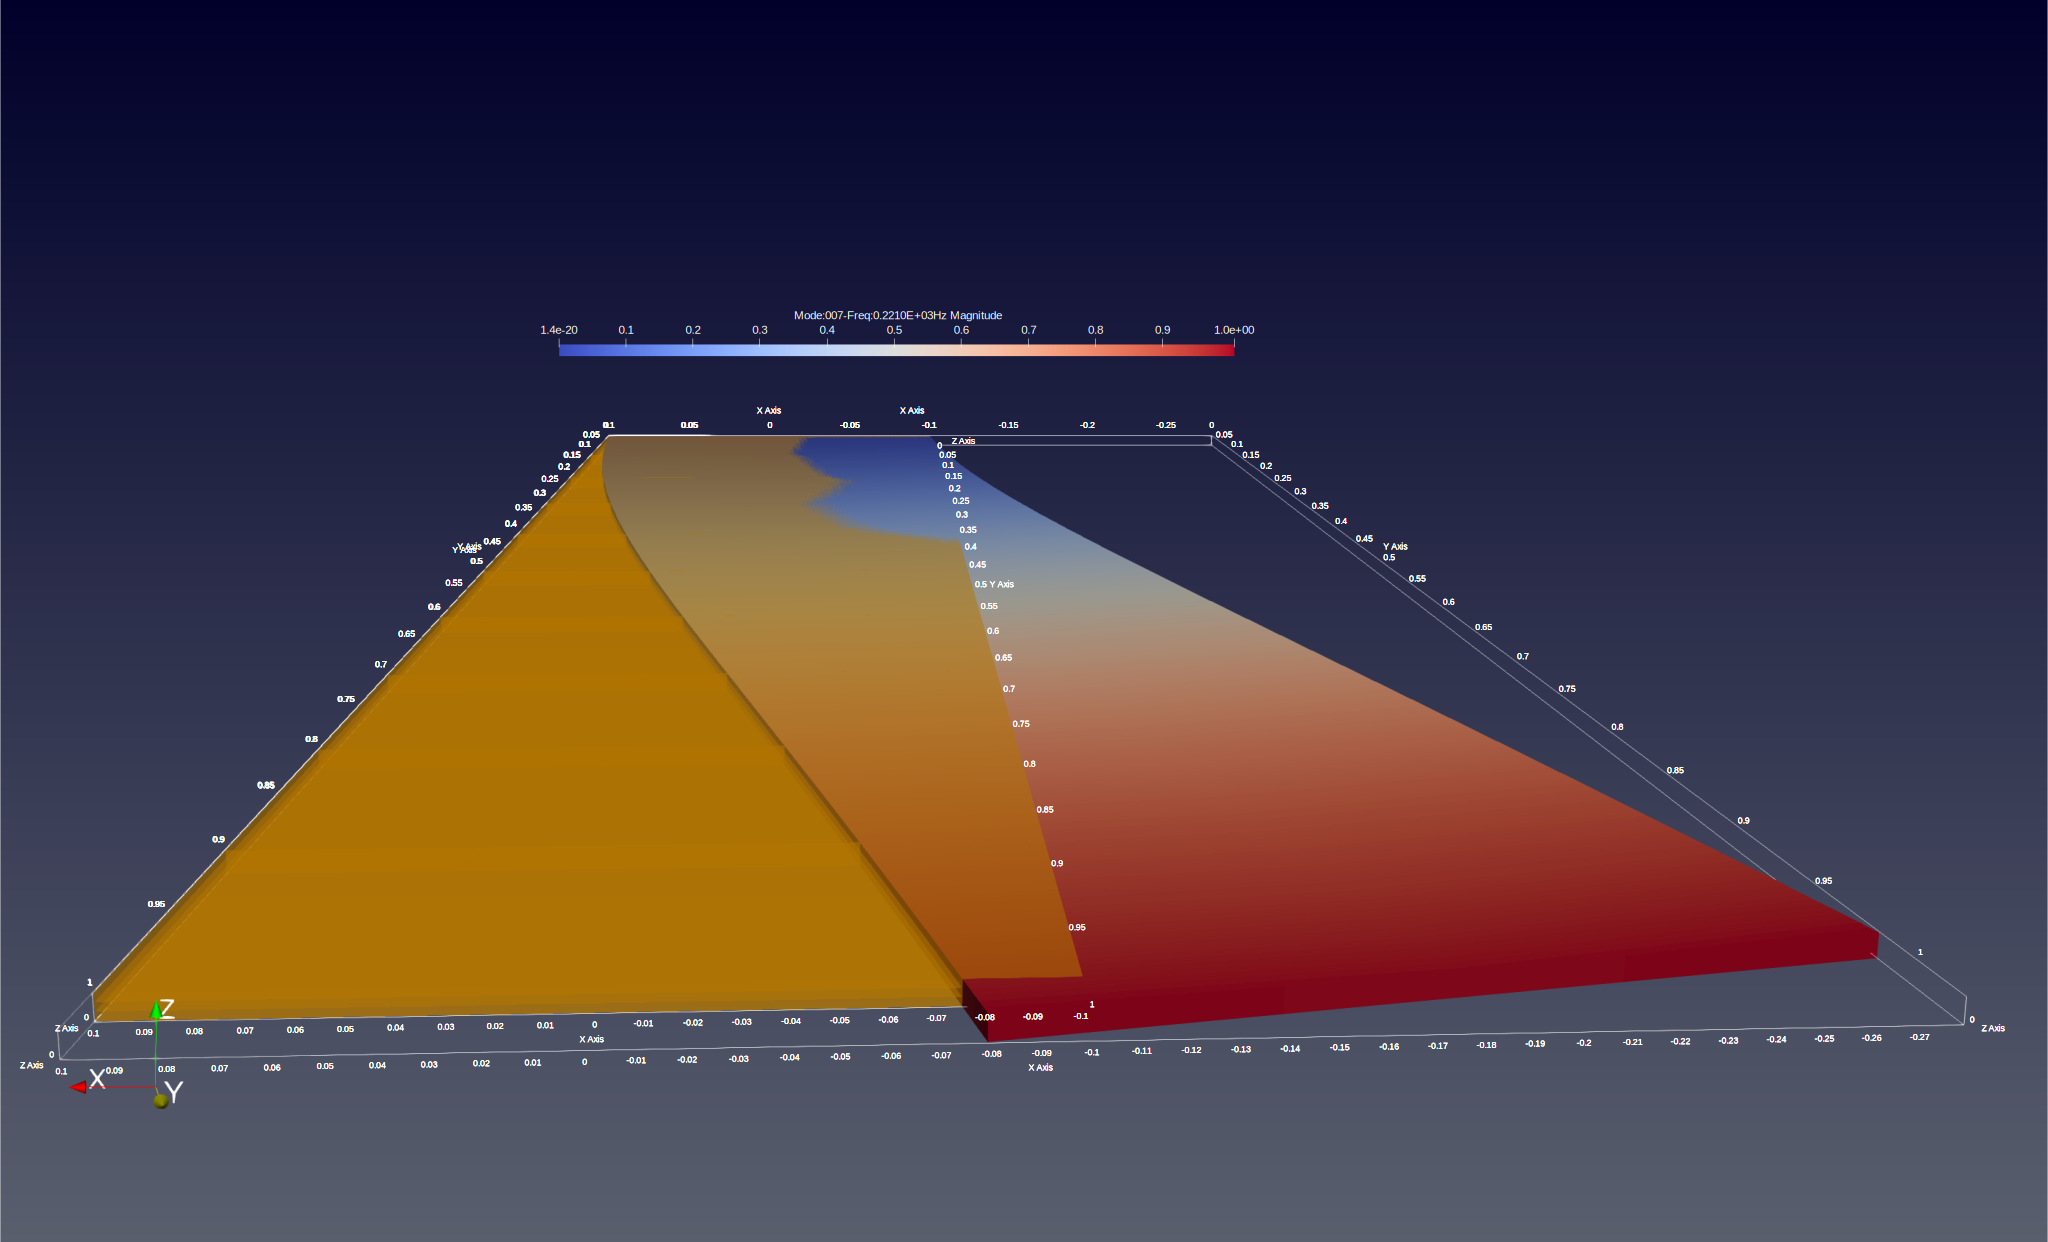
\includegraphics[width=0.5\textwidth]{MUL2/Esercitazione3/MUL2_FEM/OUTPUT/dynamic/90deg/Flex/flex5.eps}
                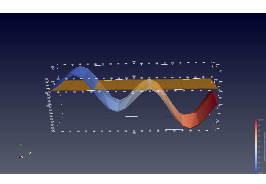
\includegraphics[width=0.5\textwidth]{MUL2/Esercitazione3/MUL2_FEM/OUTPUT/dynamic/90deg/Flex/flex6.eps}
                \caption{Modi propri di vibrare flessionali, laminazione a $90^\circ$}
            \end{figure}

            Si puó immediatamente notare che, all'aumentare del numero d'ordine di frequenza naturale, 
            si ha un aumento del numero di semionde di flessione.

            Fa eccezione il grado a cui corrisponde la frequenza $f_7$, per la quale si verifica una deflessione planare.

            \clearpage

            \begin{figure}[h!]
                \phantomsection \label{fig:freq_nat_torque_90}
                \includegraphics[width=0.5\textwidth]{MUL2/Esercitazione3/MUL2_FEM/OUTPUT/dynamic/90deg/Torque/torque1.eps}
                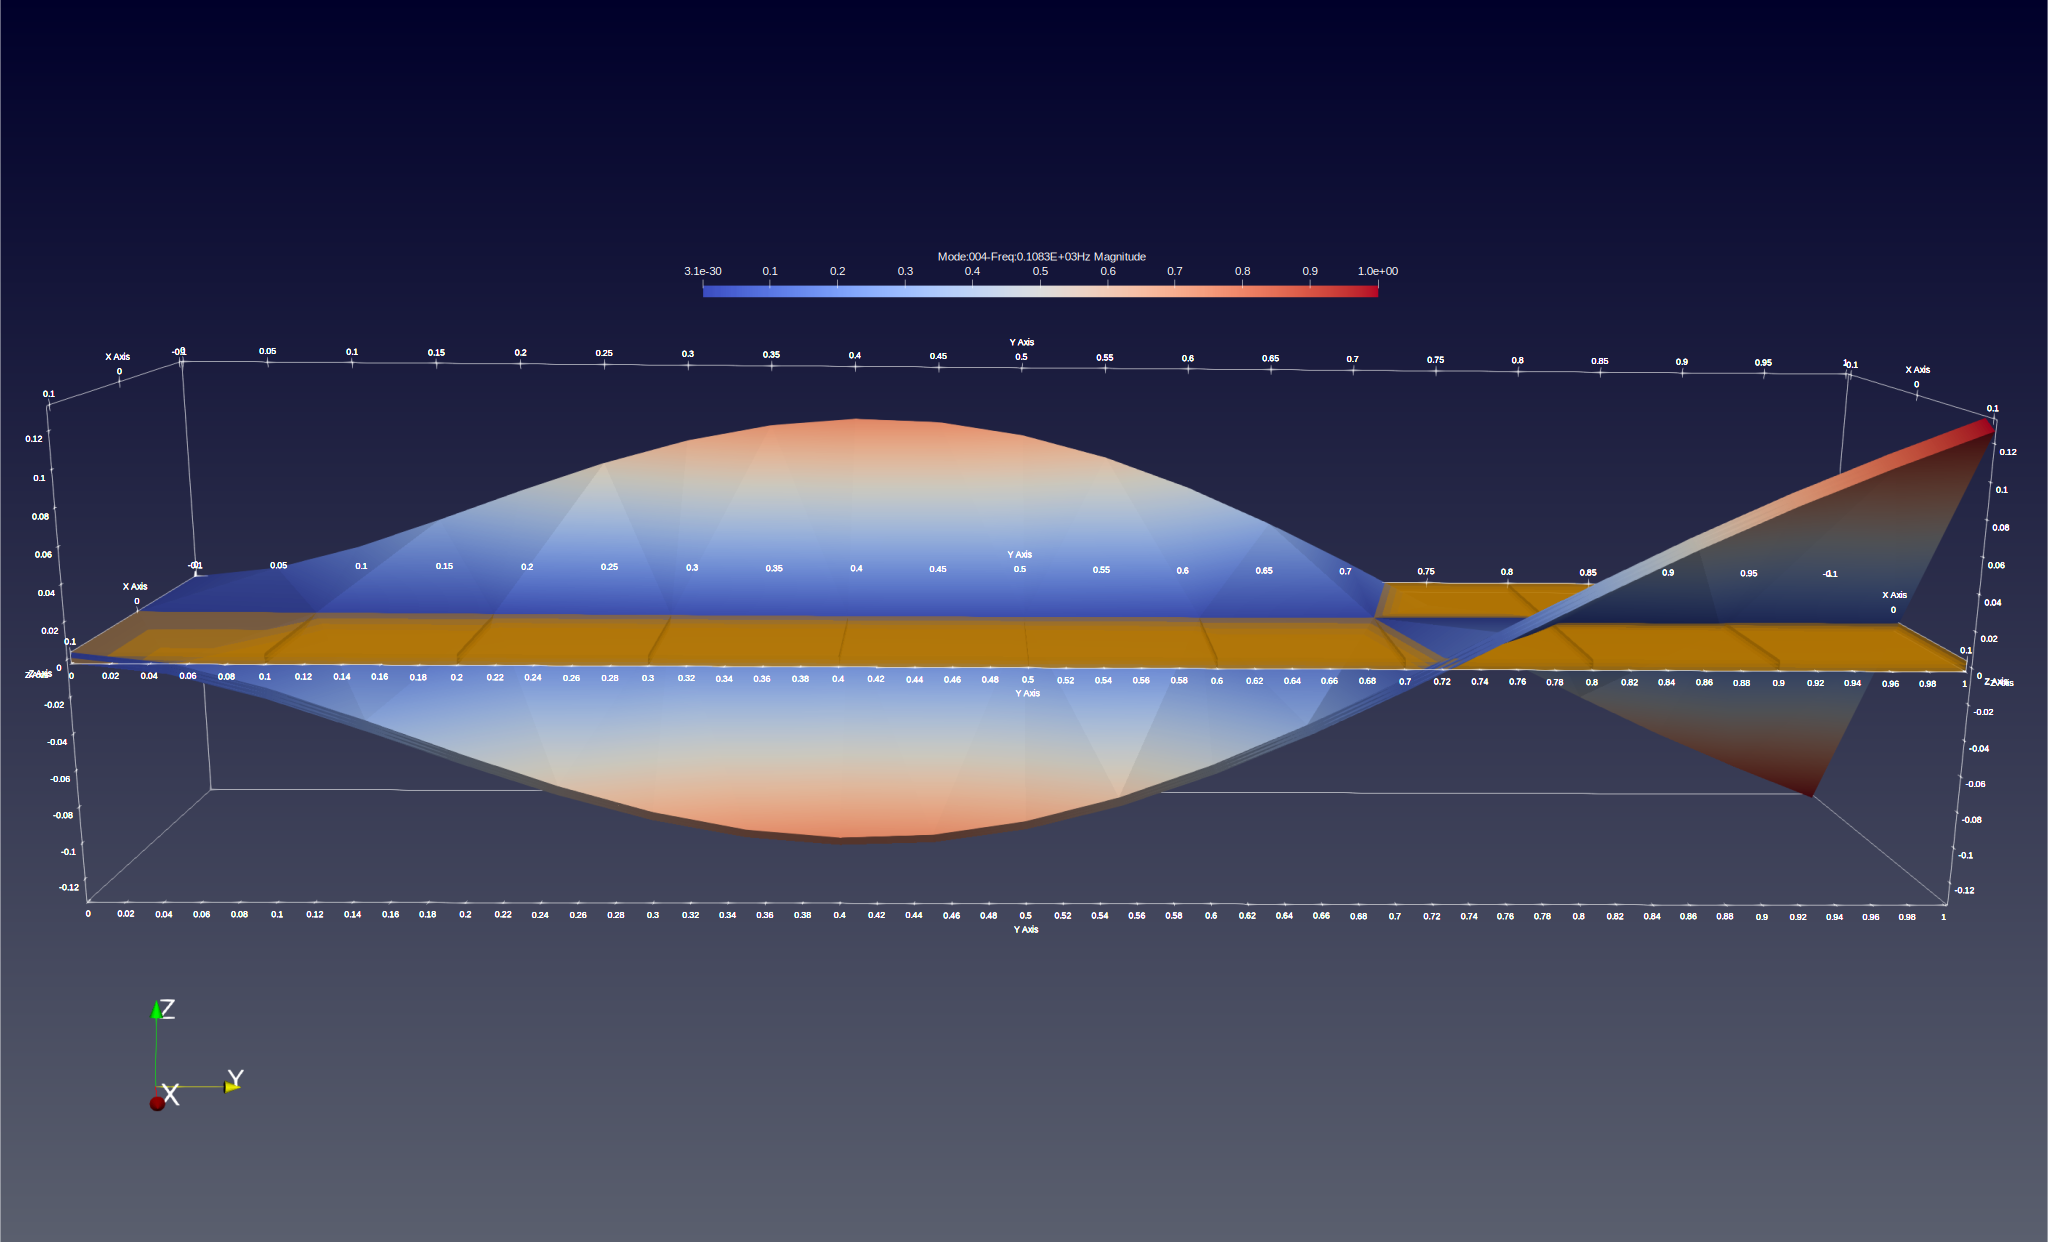
\includegraphics[width=0.5\textwidth]{MUL2/Esercitazione3/MUL2_FEM/OUTPUT/dynamic/90deg/Torque/torque2.eps}
                \includegraphics[width=0.5\textwidth]{MUL2/Esercitazione3/MUL2_FEM/OUTPUT/dynamic/90deg/Torque/torque3.eps}
                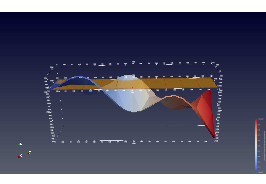
\includegraphics[width=0.5\textwidth]{MUL2/Esercitazione3/MUL2_FEM/OUTPUT/dynamic/90deg/Torque/torque4.eps}
                \caption{Modi propri di vibrare torsionali, laminazione a $90^\circ$}
            \end{figure}

            Analogamente a quanto visto per i modi di vibrare flessionali, si riscontra un aumento di semionde anche 
            nel caso relativo alla torsione.

            \clearpage

            \subsubsection{Laminazione a 45 gradi \label{Esercitazione3_freq_nat_45}}

            \begin{table}[h!]
                \centering
                \begin{tabular}{@{}ll@{}}
                \toprule
                $f_1$    & 0.896269770E+01  \ Hz \ (flex) \\
                $f_2$    & 0.347435712E+02  \ Hz \ (torque) \\
                $f_3$    & 0.559455115E+02  \ Hz \ (flex) \\
                $f_4$    & 0.114966962E+03  \ Hz \ (torque) \\
                $f_5$    & 0.155772133E+03  \ Hz \ (flex) \\
                $f_6$    & 0.224831941E+03  \ Hz \ (torque) \\
                $f_7$    & 0.237404462E+03  \ Hz \ (flex) \\
                $f_8$    & 0.302721670E+03  \ Hz \ (flex) \\
                $f_9$    & 0.374516568E+03  \ Hz \ (flex) \\
                $f_{10}$ & 0.497551402E+03  \ Hz \ (torque) \\ \bottomrule
            \end{tabular}
            \caption{Frequenze naturali}
            \label{tab:freq_nat_45}
            \end{table}
        
        Come fatto prima si visualizzano le deformazioni con \textit{Paraview} \autocite{Paraview}. 

        \clearpage

        \begin{figure}[h!]
            \phantomsection \label{fig:freq_nat_flex_45}
            \includegraphics[width=0.5\textwidth]{MUL2/Esercitazione3/MUL2_FEM/OUTPUT/dynamic/45deg/Flex/flex1_45.eps}
            \includegraphics[width=0.5\textwidth]{MUL2/Esercitazione3/MUL2_FEM/OUTPUT/dynamic/45deg/Flex/flex2_45.eps}
            \includegraphics[width=0.5\textwidth]{MUL2/Esercitazione3/MUL2_FEM/OUTPUT/dynamic/45deg/Flex/flex3_45.eps}
            \includegraphics[width=0.5\textwidth]{MUL2/Esercitazione3/MUL2_FEM/OUTPUT/dynamic/45deg/Flex/flex4_45.eps}
            \includegraphics[width=0.5\textwidth]{MUL2/Esercitazione3/MUL2_FEM/OUTPUT/dynamic/45deg/Flex/flex5_45.eps}
            \includegraphics[width=0.5\textwidth]{MUL2/Esercitazione3/MUL2_FEM/OUTPUT/dynamic/45deg/Flex/flex6_45.eps}
            \caption{Modi propri di vibrare flessionali, laminazione a $45^\circ$}
        \end{figure}

        Le considerazioni in merito alle semionde fatte per il caso a 90 gradi valgono anche cambiando la laminazione.

        Si puó peró notare che gli effetti della laminazione a 45 gradi tendono a far ripiegare la piastra
        su sé stessa, lungo l'asse longitudinale e l'effetto diventa man mano piú visibile con l'aumentare del grado di 
        frequenza propria.

        \clearpage

        \begin{figure}[h!]
            \phantomsection \label{fig:freq_nat_torque_45}
            \includegraphics[width=0.5\textwidth]{MUL2/Esercitazione3/MUL2_FEM/OUTPUT/dynamic/45deg/Torque/torque1_45.eps}
            \includegraphics[width=0.5\textwidth]{MUL2/Esercitazione3/MUL2_FEM/OUTPUT/dynamic/45deg/Torque/torque2_45.eps}
            \includegraphics[width=0.5\textwidth]{MUL2/Esercitazione3/MUL2_FEM/OUTPUT/dynamic/45deg/Torque/torque3_45.eps}
            \includegraphics[width=0.5\textwidth]{MUL2/Esercitazione3/MUL2_FEM/OUTPUT/dynamic/45deg/Torque/torque4_45.eps}
            \caption{Modi propri di vibrare torsionali, laminazione a $45^\circ$}
        \end{figure}

        Quanto detto per la laminazione a 90 gradi rimane valido e, come giá messo in evidenza poc'anzi, 
        la laminazione a 45 gradi causa un crescente ripiegamento lungo l'asse longitudinale, tuttavia piú visibile
        nei gradi flessionali.

        
        

            \clearpage

            \subsection{Analisi Statica: displacement massimo \label{displacement_massimo}}

            Supponendo un carico di 200 N, agente ortogonalmente sull'estremo libero della piastra, si visualizza il massimo displacement
            lungo l'asse z, calcolato dallo script in Fotran menzionato nella sezione \ref{Esercitazione3_freq_nat}, con modello LE.

            Anche i dati di riferimento per le successive analisi statiche e termiche sono output dello stesso script, per il quale vengono opportunamente
            modificati i file di input.

            \subsubsection{Laminazione a 90 gradi \label{displacement_massimo_90}}

            \begin{figure}[h!]
                \phantomsection \label{fig:displacement_90}
                \centering
                \includegraphics[width=0.7\textwidth]{MUL2/Esercitazione3/MUL2_FEM/OUTPUT/static/Displacement_Z/displacement_static_90.eps}
                \caption{Displacement massimo, pari a $1.4 \cdot 10^{-1} \ m$}
            \end{figure}


            \subsubsection{Laminazione a 45 gradi \label{displacement_massimo_45}}

            \begin{figure}[h!]
                \phantomsection \label{fig:displacement_45}
                \centering
                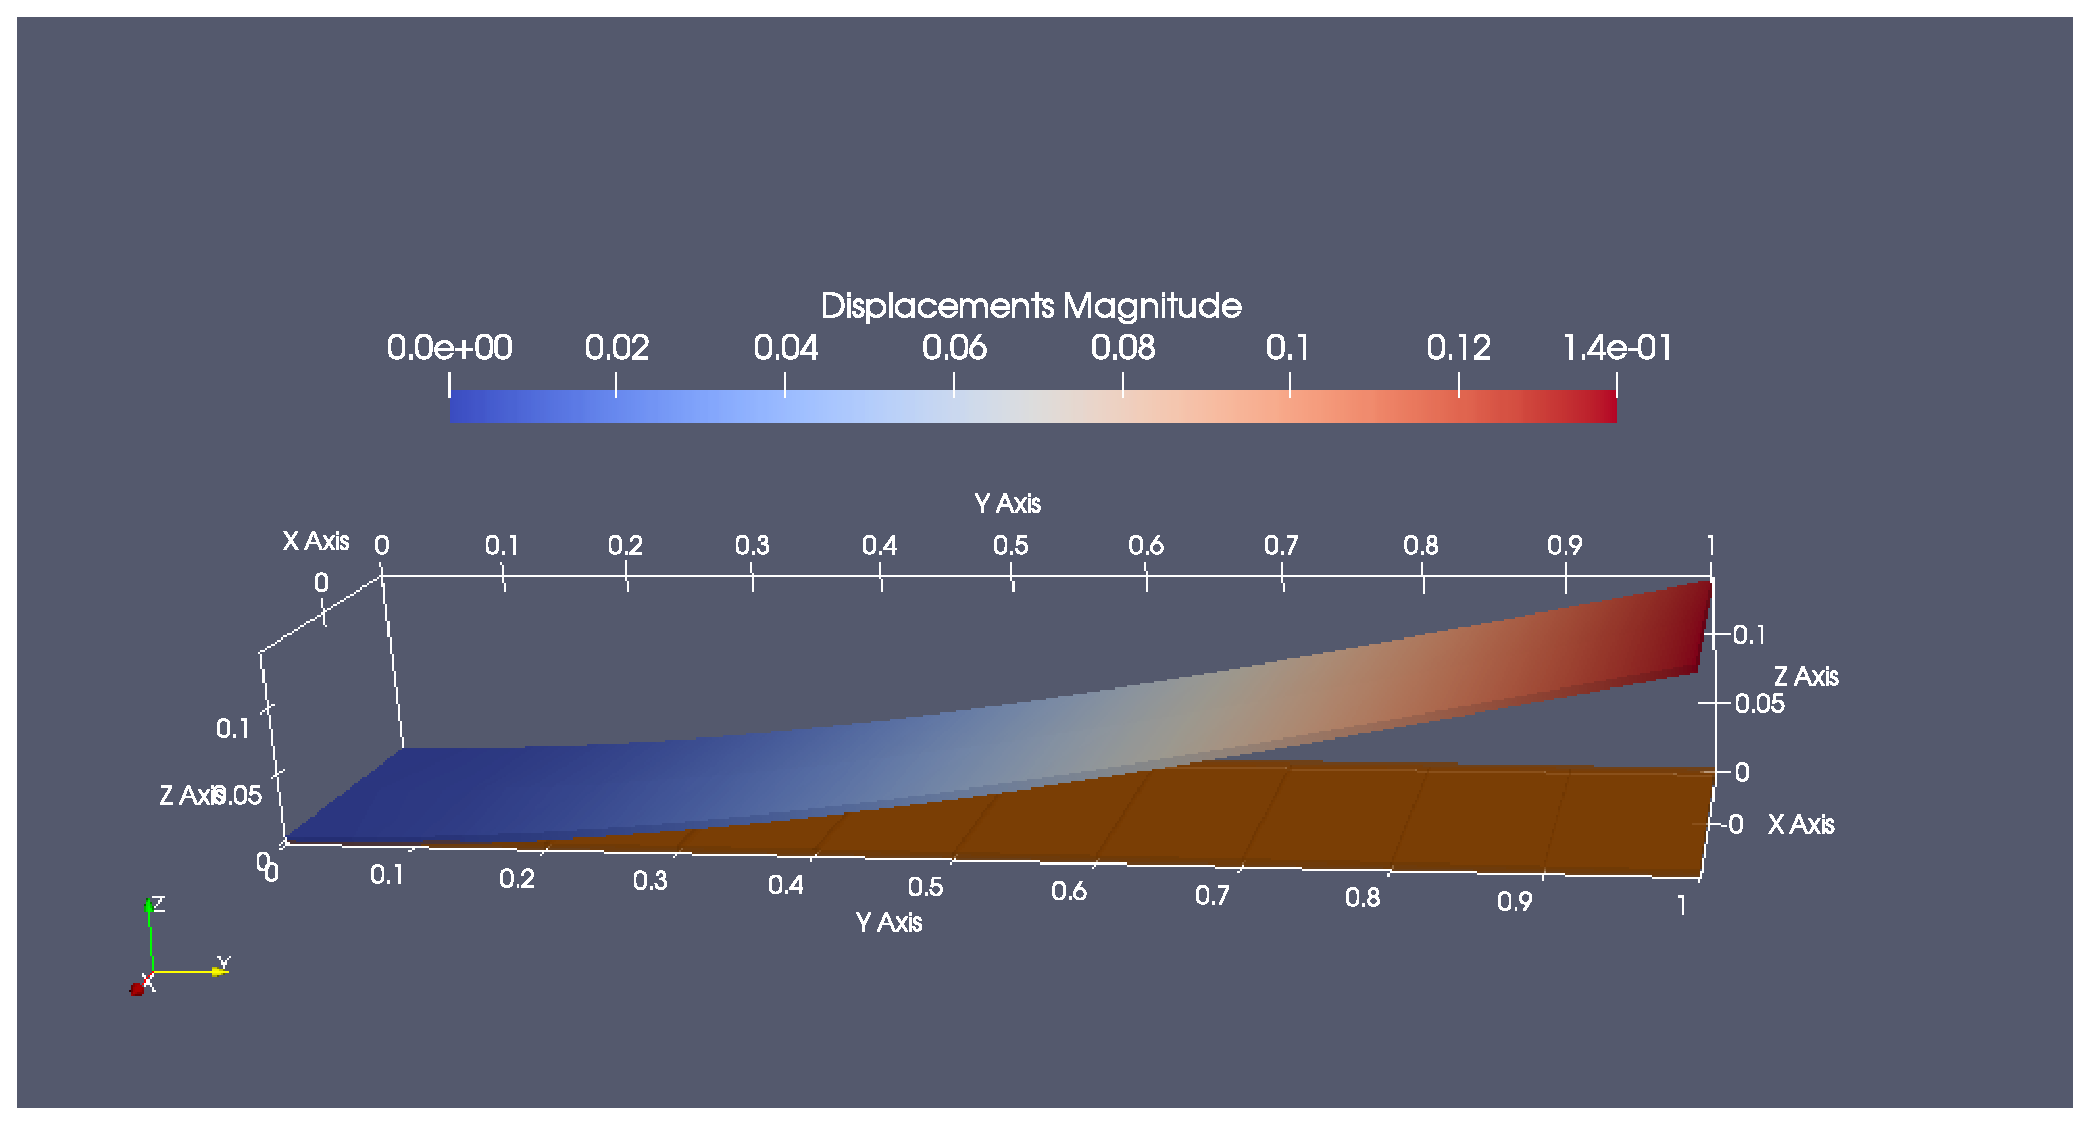
\includegraphics[width=0.7\textwidth]{MUL2/Esercitazione3/MUL2_FEM/OUTPUT/static/Displacement_Z/displacement_static_45.eps}
                \caption{Displacement massimo, pari a $1.4 \cdot 10^{-1} \ m$}
            \end{figure}

            \clearpage

            \subsection{Analisi statica: distribuzione degli stress \label{statica_stress}}

            Attraverso uno script in \textit{Octave} \autocite{Octave}, disponibile sul repository di questo report \autocite{Esercitazioni_strutture}
            col nome di \textit{Plot\_sigmas.m}, tutti gli stress richiesti, ottenuti come output dell'analisi statica e dell'analisi termica (per laminazione a 90 e 45 gradi)
            vengono plottati lungo lo spessore z in corrispondenza del baricentro, prestando attenzione alla differenza tra il modello lagrangiano LE
            e il modello di Taylor TE, quest'ultimo iterato dal primo fino al sesto grado del polinomio approssimante.

            \subsubsection{Laminazione a 90 gradi\label{statica_stress_90}}

            \begin{figure}[h!]
                \phantomsection \label{fig:sigmas_static_90}
                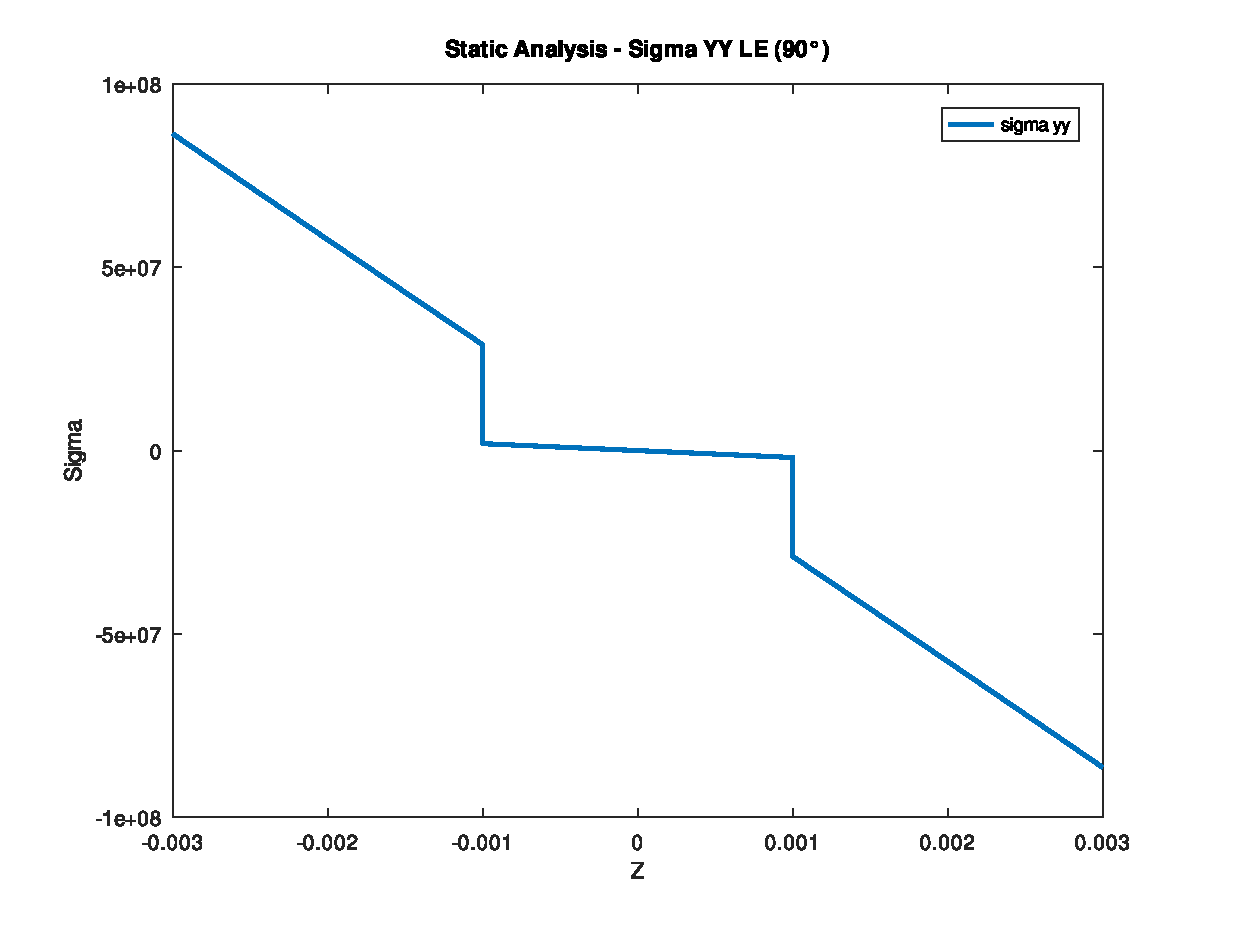
\includegraphics[width=0.5\textwidth]{MUL2/Esercitazione3/MUL2_FEM/OUTPUT/PLOT/static_YY_LE_90.svg.eps}
                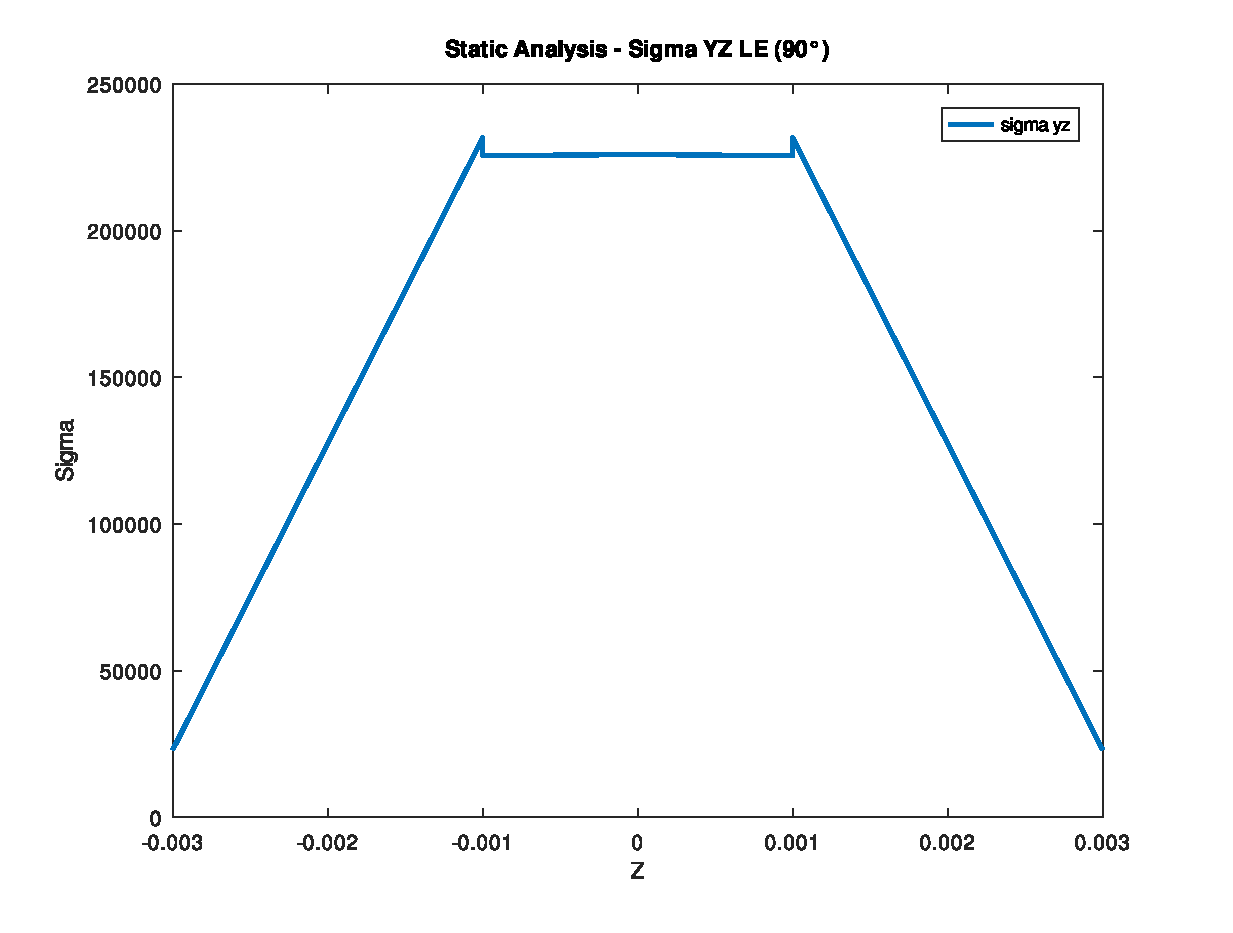
\includegraphics[width=0.5\textwidth]{MUL2/Esercitazione3/MUL2_FEM/OUTPUT/PLOT/static_YZ_LE_90.svg.eps}
                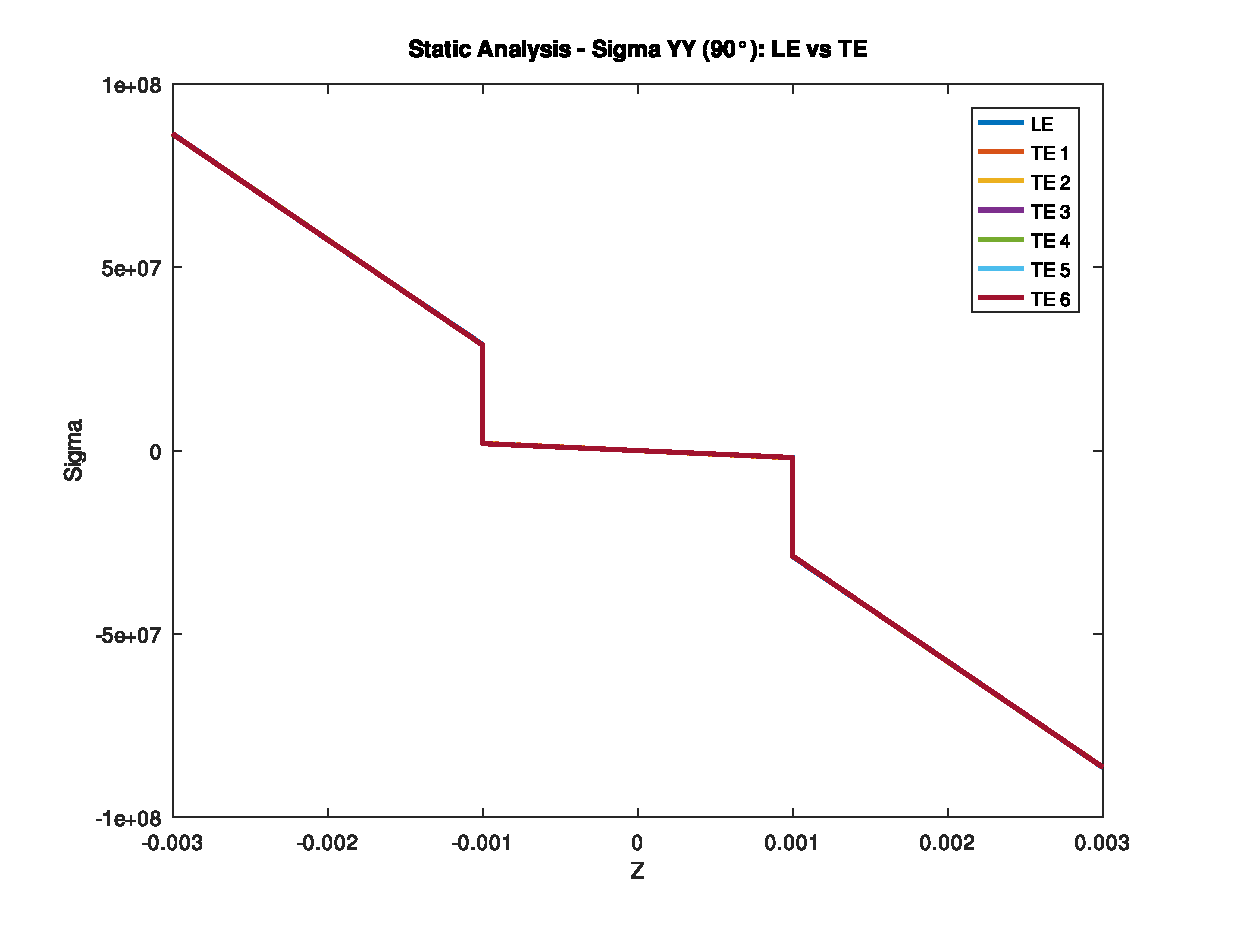
\includegraphics[width=0.5\textwidth]{MUL2/Esercitazione3/MUL2_FEM/OUTPUT/PLOT/static_YY_LEvsTE_90.svg.eps}
                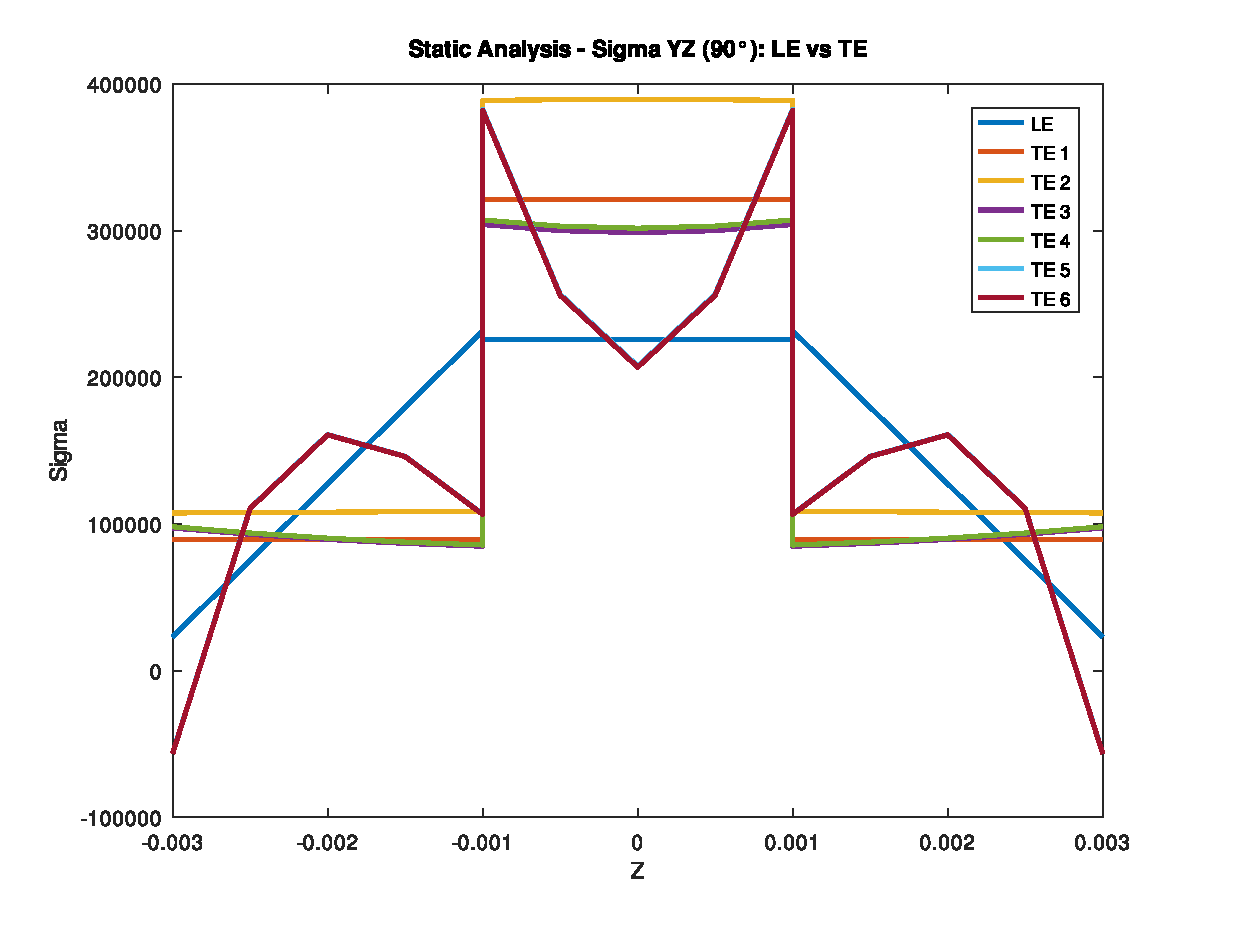
\includegraphics[width=0.5\textwidth]{MUL2/Esercitazione3/MUL2_FEM/OUTPUT/PLOT/static_YZ_LEvsTE_90.svg.eps}
                \caption{Sigma YY e Sigma YZ, modelli LE e TE a confronto}
            \end{figure}

            Si notano delle discontinuitá (di varia entitá a seconda dello stress e del modello considerato) lungo lo spessore,
            in prossimitá del baricentro, poiché la lamina centrale ha un orientamento diverso, per cui la piastra presenta rigidezze
            diverse nella stessa direzione. Inoltre, per quanto riguarda la $\sigma_{yy}$, il risultato di tutti i modelli
            é praticamente coincidente, per cui un'approssimazione al primo ordine ha giá la massima accuratezza desiderabile.
            Invece, per quanto riguarda la $\sigma_{yz}$, la precisione aumenta con l'incremento di grado del polinomio, tendendo
            man mano all'andamento del metodo lagrangiano. Si evidenzia infine un'inversione al centro della piastra,
            dovuta alla laminazione.

            \clearpage 

            \subsubsection{Laminazione a 45 gradi\label{statica_stress_45}}

            \begin{figure}[h!]
                \phantomsection \label{fig:sigmas_static_45}
                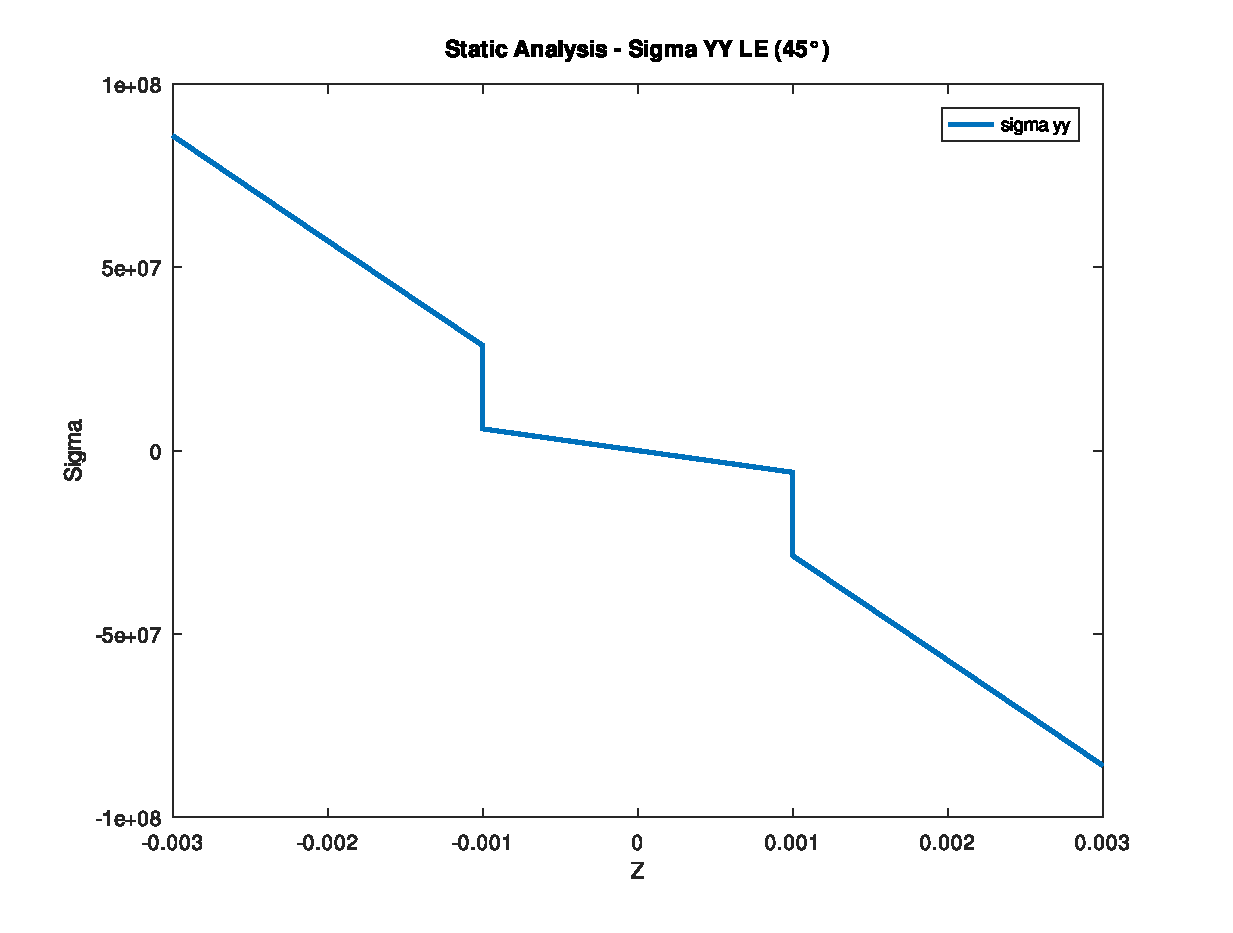
\includegraphics[width=0.5\textwidth]{MUL2/Esercitazione3/MUL2_FEM/OUTPUT/PLOT/static_YY_LE_45.svg.eps}
                \includegraphics[width=0.5\textwidth]{MUL2/Esercitazione3/MUL2_FEM/OUTPUT/PLOT/static_YZ_LE_45.svg.eps}
                \includegraphics[width=0.5\textwidth]{MUL2/Esercitazione3/MUL2_FEM/OUTPUT/PLOT/static_YY_LEvsTE_45.svg.eps}
                \includegraphics[width=0.5\textwidth]{MUL2/Esercitazione3/MUL2_FEM/OUTPUT/PLOT/static_YZ_LEvsTE_45.svg.eps}
                \caption{Sigma YY e Sigma YZ, modelli LE e TE a confronto}
            \end{figure}

            Rispetto alla laminazione a 90 gradi, sebbene gli andamenti siano generalmente simili, si evidenzia in 
            $\sigma_{yy}$ un leggero discostamento dal modello LE, apprezzabile solo per quanto riguarda il polinomio di primo grado.

            L'andamento di $\sigma_{yz}$ rispecchia in buona parte il precedente, con una magnitudine peró inferiore nell'intorno
            del baricentro e con un'inversione solo nel polinomio di sesto grado.

            \clearpage


            \subsection{Analisi Termica: displacement massimo \label{displacement_massimo_thermal}}

            Si procede con un'analisi termica, con la stessa procedura vista per l'analisi statica. Tuttavia,
            si utilizza questa volta un carico termico pari a 120 C. 

            \subsubsection{Laminazione a 90 gradi \label{displacement_massimo_90_thermal}}

            \begin{figure}[h!]
                \phantomsection \label{fig:displacement_90_thermal}
                \centering
                \includegraphics[width=0.7\textwidth]{MUL2/Esercitazione3/MUL2_FEM/OUTPUT/static/Displacement_Z/displacement_thermal_90.eps}
                \caption{Displacement massimo, pari a $1.4 \cdot 10^{-1} \ m$}
            \end{figure}


            \subsubsection{Laminazione a 45 gradi \label{displacement_massimo_45_thermal}}

            \begin{figure}[h!]
                \phantomsection \label{fig:displacement_45_thermal}
                \centering
                \includegraphics[width=0.7\textwidth]{MUL2/Esercitazione3/MUL2_FEM/OUTPUT/static/Displacement_Z/displacement_thermal_45.eps}
                \caption{Displacement massimo, pari a $1.4 \cdot 10^{-1} \ m$}
            \end{figure}

            A differenza dell'analisi statica, non si ha un displacement lungo z, ma solo una dilatazione volumica dovuta
            al carico termico, apprezzabile come displacement massimo lungo y.

            La laminazione a 45 gradi fa sí che la dilatazione si sviluppi comunque in maniera preponderante lungo y, 
            ma con una una deviazione planare lungo l'asse x.

            \clearpage

            \subsection{Analisi Termica: distribuzione degli stress \label{termica_stress}}

            Si analizzano in questo caso gli stress normali $\sigma_{xx}$, $\sigma_{yy}$, $\sigma_{zz}$.

            \subsubsection{Laminazione a 90 gradi\label{termica_stress_90}}

            \begin{figure}[h!]
                \centering
                \phantomsection \label{fig:sigmas_thermal_90}
                \includegraphics[width=0.3\textwidth]{MUL2/Esercitazione3/MUL2_FEM/OUTPUT/PLOT/thermal_XX_LE_90.svg.eps}
                \includegraphics[width=0.3\textwidth]{MUL2/Esercitazione3/MUL2_FEM/OUTPUT/PLOT/thermal_YY_LE_90.svg.eps}
                \includegraphics[width=0.3\textwidth]{MUL2/Esercitazione3/MUL2_FEM/OUTPUT/PLOT/thermal_ZZ_LE_90.svg.eps}
                \includegraphics[width=0.3\textwidth]{MUL2/Esercitazione3/MUL2_FEM/OUTPUT/PLOT/thermal_XX_LEvsTE_90.svg.eps}
                \includegraphics[width=0.3\textwidth]{MUL2/Esercitazione3/MUL2_FEM/OUTPUT/PLOT/thermal_YY_LEvsTE_90.svg.eps}
                \includegraphics[width=0.3\textwidth]{MUL2/Esercitazione3/MUL2_FEM/OUTPUT/PLOT/thermal_ZZ_LEvsTE_90.svg.eps}
                \caption{Sigma XX, Sigma YY e Sigma ZZ, modelli LE e TE a confronto}
            \end{figure}

            A conferma di quanto giá visto in sezione \ref{displacement_massimo_thermal}, lo stress $\sigma_{yy}$
            é piú grande degli altri di ben due ordini di grandezza, dato che la direzione y e quella piú sollecitata.

            Inoltre, analogamente a quanto visto per l'analisi statica, la laminazione a 90 gradi fa sí che il layer 
            centrale presenti, nell'intorno del baricentro, un picco negativo di sollecitazione, dovuto all'orientamento delle fibre. \\ 

            Infine, le considerazioni fatte per l'analisi statica e il confronto tra i modelli TE ed LE valgono anche per l'analisi termica.
            
            All'aumentare del grado del polinomio approssimante del modello di Taylor, si ha un andamento man mano piú fedele a quello ottenuto 
            col modello lagrangiano, in cui, per $\sigma_{xx}$, solo il sesto grado riesce ad approssimare con discreta accuratezza
            l'avvallamento centrale.

            
        

            \clearpage 

            \subsubsection{Laminazione a 45 gradi\label{termica_stress_45}}

            \begin{figure}[h!]
                \centering
                \phantomsection \label{fig:sigmas_thermal_45}
                \includegraphics[width=0.3\textwidth]{MUL2/Esercitazione3/MUL2_FEM/OUTPUT/PLOT/thermal_XX_LE_45.svg.eps}
                \includegraphics[width=0.3\textwidth]{MUL2/Esercitazione3/MUL2_FEM/OUTPUT/PLOT/thermal_YY_LE_45.svg.eps}
                \includegraphics[width=0.3\textwidth]{MUL2/Esercitazione3/MUL2_FEM/OUTPUT/PLOT/thermal_ZZ_LE_45.svg.eps}
                \includegraphics[width=0.3\textwidth]{MUL2/Esercitazione3/MUL2_FEM/OUTPUT/PLOT/thermal_XX_LEvsTE_45.svg.eps}
                \includegraphics[width=0.3\textwidth]{MUL2/Esercitazione3/MUL2_FEM/OUTPUT/PLOT/thermal_YY_LEvsTE_45.svg.eps}
                \includegraphics[width=0.3\textwidth]{MUL2/Esercitazione3/MUL2_FEM/OUTPUT/PLOT/thermal_ZZ_LEvsTE_45.svg.eps}
                \caption{Sigma XX, Sigma YY e Sigma ZZ, modelli LE e TE a confronto}
            \end{figure}

            La laminazione a 45 gradi, in questo caso, produce degli effetti abbastanza visibili sull'andamento 
            degli stress normali. 

            In primo luogo, sebbene l'andamento di $\sigma_{yy}$ e $\sigma_{zz}$ siano comparabili con quelli della laminazione a 90 gradi, si nota immediatamente che 
            $\sigma_{xx}$ ha un andamento sostanzialmente diverso, oltretutto con picchi piú grandi di un ordine di grandezza. 

            Questo andamento é coerente con quanto osservato in sezione \ref{displacement_massimo_45_thermal}, dato che rispetto alla laminazione
            a 90 gradi, si ha una deviazione verso l'asse x, nel primo caso del tutto assente, come visibile in \ref{displacement_massimo_90_thermal}. \\ 

            Infine, continua a valere la migliore approssimazione dell'andamento lagrangiano da parte di polinomi di Taylor 
            di grado piú elevato.

            Tuttavia, si osserva come, nel caso di $\sigma_{xx}$ e $\sigma_{yy}$, l'approssimazione del polinomio di primo grado
            sia molto grossolana, con quasi un ordine di grandezza di errore, mentre i gradi dal secondo in poi si avvicinano in maniera
            molto precisa all'andamento target.
            


            \clearpage            
        
        \section{Esercitazione 4\label{Esercitazione4}}

        


                
        \clearpage
        \printbibliography
\end{document}